\documentclass[11pt]{article}
\usepackage[a4paper,margin=1in]{geometry}
\usepackage{amsmath,amssymb,amsthm,mathtools}
\usepackage[expansion=false]{microtype}
\usepackage{graphicx,booktabs,array}
\usepackage[font=small,labelfont=bf]{caption}
\usepackage[dvipsnames]{xcolor}
\usepackage{enumitem}
\usepackage{needspace}
\usepackage[hidelinks,pdfusetitle]{hyperref}
\usepackage[nameinlink,capitalise]{cleveref}
\setlist{nosep,leftmargin=1.5em}
\newtheorem{theorem}{Theorem}[section]
\newtheorem{lemma}[theorem]{Lemma}
\newtheorem{proposition}[theorem]{Proposition}
\newtheorem{corollary}[theorem]{Corollary}
\newtheorem{conjecture}{Conjecture}
\theoremstyle{definition}\newtheorem{definition}[theorem]{Definition}
\theoremstyle{remark}\newtheorem{remark}[theorem]{Remark}
\newcommand{\R}{\mathbb R}\newcommand{\C}{\mathbb C}\newcommand{\N}{\mathbb N}
\newcommand{\dd}{\,\mathrm d}\newcommand{\e}{\mathrm e}
\newcommand{\Num}{\mathrm{Num}}\newcommand{\Den}{\mathrm{Den}}
\renewcommand{\Re}{\operatorname{Re}}\renewcommand{\Im}{\operatorname{Im}}
\setlength{\parskip}{0.35em}
\AtBeginDocument{\sloppy}
\urlstyle{same}
\hypersetup{pdftitle={What a Zero Is: One Involution across Mathematics, Physics, Chemistry, Neuroscience, Computation and the Giant Planets},pdfauthor={Abhijit Singh}}
\title{\textbf{What a Zero Is}\\[4pt]
\large One Involution across Mathematics, Physics, Chemistry, Neuroscience, Computation and the Giant Planets}
\author{Abhijit Singh}
\date{25 September 2026}
\begin{document}
\maketitle
\begin{abstract}
The Triad Principle has four clauses: a pair $s,-s$ whose sum is the zero; the self-stable triad $\{-s,0,s\}$; the merge of units under positive coupling, which keeps the structure; and the fourth element, the observer, which becomes a member of a new triad. We state the principle as one involution $\iota$, under which every object splits into an even part, the common and reversible half, and an odd part, the difference that an observation of \emph{which member} determines; a zero is where the odd part vanishes, the balance of a pair $s,-s$. We prove each clause as a proposition: the splitting is unique exactly away from characteristic $2$; a reading of which member of a two-state pair is occupied has mean equal to twice the odd part $\delta=-\frac12\tanh(\varepsilon/2)$; the triad $\{-1,0,1\}$ is the only finite set of integers that contains $0$ and a nonzero element and is closed under negation and multiplication, and its generating function vanishes exactly at $\frac13$ and $\frac23$ of a turn; the merge of two elementary pairs under a coupling $\kappa\ge0$ keeps both zeros on the unit circle and is the uniform triad exactly at $\kappa=\frac12\ln2$, while $\kappa<0$ sends them off the circle as a mirrored pair; and a probe qubit reading a triad decoheres completely at $\frac13$ and $\frac23$ of its period, its record a new balanced triad. We then give the exact instance of every clause in each of seven field papers, in mathematics, physics, quantum theory, chemistry, neuroscience, computation and planetary science, and collect them in one correspondence, from the signed current $J$ of Riemann's $\xi$, whose positivity is equivalent to the Riemann Hypothesis (RH) and is proved outside an explicit region, to the NH$_4$SH titration whose zero at $\mathrm{N/S}=1$ decides which ice tops each giant planet. Five structures recur as identities across the set: the two-state law $p=1/(1+\e^{\varepsilon})$ with odd part $-\frac12\tanh(\varepsilon/2)$; the triad generating function $z^{-1}+1+z$; one merge rule for zeros; the Klein four-group generated by an involution and complex conjugation, whose orbits collapse to pairs exactly on the critical line, on the imaginary axis of a Hamiltonian spectrum and on the Lee--Yang circle; and one observer, whose complete-decoherence times are the Lee--Yang zeros of what it reads.

For $\xi$ the involution is $s\mapsto1-s$. It comes from Poisson summation, which also gives the modular invariance of the closed string and T-duality, and its automorphic form is the invariance of the Eisenstein series under $\tau\mapsto-1/\tau$: the Wigner function of Riemann's kernel is an explicit operator applied to $E^*(i\e^p,\frac12+ix)$ that removes exactly its two constant terms. We give seven readings of a zero: a balance of two halves of $0.158$ each, equal to within $4\times10^{-15}$ at the first three zeros; a phase vortex of winding number one; a Lee--Yang zero, with all $12$--$14$ zeros of two ferromagnetically coupled Riemann spins below height $40$ on the imaginary axis while the Epstein control loses $4$ of $7$; a scattering resonance, $|\varphi|=1$ on the unitary line to $2\times10^{-13}$; a spectral level, the $22{,}491$ zeros below $2\times10^4$ at $L^1$ distance $0.073$ from GUE; a mass; and the time of a dynamical phase transition. In the set RH is equivalent to $J\ge0$ on the remaining region and to six further statements, and any proof of it must use a property that $\zeta$ has and the Epstein zeta function lacks, such as the Euler product. The propositions are proved by exact algebra and the Lee--Yang circle theorem; the readings are computed by quadrature, Euler--Maclaurin summation, the Riemann--Siegel formula and the argument principle.
\end{abstract}

\tableofcontents

\section{Introduction}\label{sec:intro}
\subsection{The principle and the zero}
\paragraph{The Triad Principle.} The Triad Principle has four clauses: \emph{the pair}, $s$ and $-s$, whose sum is the zero; \emph{the triad} $\{-s,0,s\}$, which is self-stable; \emph{the merge} of units under positive coupling, which keeps the structure; and \emph{the fourth} element, the observer of a triad, which itself becomes a member of a new triad. This paper states the principle as one involution $\iota$, proves each clause in exact form (\cref{sec:principle}), and shows how each of the seven field papers \cite{SMath,SPhys,SQuant,SChem,SNeuro,SAlg,SPlanet} realises each clause (\cref{sec:fields}). We refer to the field papers by their numbers in the set:
\begin{itemize}
\item 01, Mathematics \cite{SMath}: \emph{Pair Balance and the Riemann Zeros};
\item 02, Physics \cite{SPhys}: \emph{The Reversible Half and the Third Body};
\item 03, Quantum \cite{SQuant}: \emph{The Riemann Kernel as a Quantum State};
\item 04, Chemistry \cite{SChem}: \emph{Which Member Carries};
\item 05, Neuroscience \cite{SNeuro}: \emph{The Balanced Pair in Excitable Tissue};
\item 06, Algorithms \cite{SAlg}: \emph{Three Is Enough};
\item 07, Planetary Science \cite{SPlanet}: \emph{The Four Giants as Balanced Pairs}.
\end{itemize}

\paragraph{What a zero is.} Riemann's function $\xi(s)=\frac12s(s-1)\pi^{-s/2}\Gamma(\frac s2)\zeta(s)$ satisfies $\xi(s)=\xi(1-s)$. In the variable $z$ of $\Xi(z)=\xi(\frac12+iz)=\int_0^\infty\Phi(\tau)\cos(z\tau)\,d\tau$, with Riemann's kernel
\[
\Phi(\tau)=4\sum_{n\ge1}\bigl(2\pi^2n^4e^{9\tau/2}-3\pi n^2e^{5\tau/2}\bigr)e^{-\pi n^2e^{2\tau}},
\]
which is even in $\tau$ (\cref{sec:poisson}), positive (for $\tau\ge0$ each term is $4\pi n^2e^{5\tau/2}(2\pi n^2e^{2\tau}-3)e^{-\pi n^2e^{2\tau}}>0$) and decays like $\exp(-\pi e^{2|\tau|})$, the involution is $z\mapsto-z$ together with reality on $\R$, and its fixed line is the real axis. The central open problem about these zeros is the following.

\begin{conjecture}[the Riemann Hypothesis]\label{conj:RH}
Every nontrivial zero of $\zeta$ lies on the line $\Re s=\frac12$, the fixed line of the reflection $s\mapsto1-\bar s$; equivalently, every zero of $\Xi$ is real.
\end{conjecture}

Write $z=x+iy$, $H=|\Xi(x+iy)|^2$, which is even in $y$, and $J=2\partial_yH$, the signed current, which is odd. \Cref{conj:RH} holds if and only if $J\ge0$ for $y>0$ \cite{SD,Lagarias,SMath}, and 01 proves $J>0$ outside the region
\[
\mathcal U=\Bigl\{|x|>3\cdot10^{12}-\tfrac12,\ \ 0<y<\tfrac12-\frac1{5.573412\log(|x|+\frac12)}\Bigr\},
\]
from the verification of RH to height $3\cdot10^{12}$ \cite{PT} and the zero-free region with constant $5.573412$ \cite{MT}. The set proves six further statements equivalent to \cref{conj:RH} and reduces it to one statement on $\mathcal U$, \cref{conj:step} (\cref{sec:rh}). Unconditional results carry the balance part of the way: the proportion of zeros proved to lie on the critical line has risen as in \cref{tab:prior}.

\begin{table}[ht]\centering\small
\caption{Lower bounds for the proportion of nontrivial zeros of $\zeta$ on the critical line.}\label{tab:prior}
\begin{tabular}{@{}llll@{}}\toprule
authors & year & proportion & note\\\midrule
Levinson \cite{Levinson} & 1974 & more than $\frac13$ & ---\\
Pratt, Robles, Zaharescu, Zeindler \cite{PRZZ} & 2020 & more than $\frac5{12}$ & ---\\
Alp\"oge, Furman \cite{AF} & 2026 & at least $0.6725$ & simple zeros; preprint\\\bottomrule
\end{tabular}
\end{table}

A zero of $\Xi$ is usually described as a number. We describe what it \emph{is}, in the sense of what vanishes and why, in seven ways (\cref{sec:zero}), and show that the same structure organises the field papers and several classical constructions in string theory and statistical mechanics.

\subsection{Main results}
Our first result states the principle in exact form.

\needspace{10\baselineskip}
\begin{theorem}[the Triad Principle in exact form]\label{thm:principle}
\leavevmode
\begin{enumerate}[label=\textup{(\alph*)}]
\item \emph{The pair.} Let $\iota$ be a linear involution of a vector space $V$ over a field $K$. If $\operatorname{char}K\ne2$, every $F\in V$ splits uniquely as $F=F_++F_-$ with $\iota F_\pm=\pm F_\pm$, and the fixed set of $\iota$ is $\{F:F_-=0\}$. If $\operatorname{char}K=2$ and $V\ne0$, no vector has a unique splitting.
\item \emph{The two-state pair.} For two members with weights $p$ and $1-p$ exchanged by $\iota$, and $\varepsilon=\ln\frac{1-p}p$, the odd part of $p$ is $\delta=p-\frac12=-\frac12\tanh(\varepsilon/2)$. A reading $X=\pm1$ of which member is occupied has $\mathbb EX=2\delta$ and variance $1-4\delta^2$. At the zero $\delta=0$ the entropy takes its maximum $\ln2$, and the occupancies $\frac13$, $\frac23$ are the pair $\varepsilon=\pm\ln2$.
\item \emph{The triad.} $T=\{-1,0,1\}$ is the only finite subset of $\mathbb Z$ that contains $0$ and a nonzero element and is closed under negation and multiplication. It is a complete residue system modulo $3$, and its generating function $z^{-1}+1+z$ vanishes exactly at $\e^{\pm2\pi i/3}$, at $\frac13$ and $\frac23$ of a turn.
\item \emph{The merge.} Let two members $\varsigma_1,\varsigma_2\in\{\pm\frac12\}$ carry the weight $\e^{4\kappa\varsigma_1\varsigma_2}$. For $\kappa\ge0$ both zeros of the generating function of $\varsigma_1+\varsigma_2$ lie on $|z|=1$; at $\kappa=\frac12\ln2$ the sum is the uniform triad; for $\kappa<0$ the zeros are a real mirrored pair $z,1/z$ off the circle. Every finite system of uniform triads with couplings $\kappa_{jk}\ge0$ has all its Lee--Yang zeros on $|z|=1$.
\item \emph{The fourth.} A probe qubit in $|{+}\rangle$ coupled to a system by $\lambda\sigma_z\otimes B$ has coherence $\frac12L(t)$ with $L(t)=\sum_bp_b\e^{-2i\lambda tb}$. For the uniform triad $L(t)=\frac13(1+2\cos2\lambda t)$ vanishes exactly at $\frac13$ and $\frac23$ of the period $\pi/\lambda$, where the three phases are the cube roots of unity and sum to zero; and if $p_m=c_m/Z(1)$ with $Z(z)=\sum_mc_mz^m$, then $L(t)=Z(\e^{-2i\lambda t})/Z(1)$, so the complete-decoherence times are the Lee--Yang zeros on the unit circle.
\end{enumerate}
\end{theorem}

Our second result is the master correspondence. \Cref{def:instance} makes precise what an instance of the principle in a field is: an involution with its even and odd parts, and exact realisations of the zero, the triad, the merge and the fourth. In each of the seven field papers every clause has such an instance, resting on a theorem or computation of that paper. \Cref{tab:master} lists them with the key result of each paper, and \cref{sec:fields} states each one.

\begin{table}[!htbp]\centering\scriptsize\setlength{\tabcolsep}{2.5pt}
\caption{The master correspondence: the Triad Principle in the seven field papers.}\label{tab:master}
\begin{tabular}{@{}>{\raggedright\arraybackslash}p{0.45cm}>{\raggedright\arraybackslash}p{2.3cm}>{\raggedright\arraybackslash}p{2.1cm}>{\raggedright\arraybackslash}p{2.3cm}>{\raggedright\arraybackslash}p{2.3cm}>{\raggedright\arraybackslash}p{2.1cm}>{\raggedright\arraybackslash}p{3.2cm}@{}}\toprule
no. & pair & zero & triad & merge & fourth & key result\\\midrule
01 & $0=s(1+(-1))$; the mirror $s\mapsto1-s$; even and odd length & the critical line; $J=0$ there; $1+1=0$ at the prime $2$ & $\mathbb Z/3$: the pair at $\frac13,\frac23$; $L(0,\chi_{-3})=\frac13$ & the Euler product; $\mathbb E[Y^s]=2\xi(s)$; mirror only at $\nu=2$ & $V_4$ of order four; the fourth configuration on the zero & RH $\iff J\ge0$; $J>0$ off $\mathcal U$; a proof must use a property $\zeta$ has and the Epstein function lacks, such as the Euler product\\[2pt]
02 & $C$ and $\tilde C$; $I_+$ and $I_-$ & detailed balance; the pulsating field & figure-eight $(-s,0,s)$ six times per period & gravity couples every pair with one sign; the eight keeps its shape, the equal triangle grows at $\omega/\sqrt2$ & fourth body; the singlet & $0\le h(S)-h(C)\le\mathrm{EP}/4$; $\delta_{\max}\simeq2.84\,\varepsilon D^{-3/2}$\\[2pt]
03 & parity of $\Phi$; $z$ and $\bar z$ & the real time axis; complete decoherence & spin-1: $L=\frac13(1+2\cos2\lambda t)$ & Ising pair at $\frac12\ln2$; chains with $K\ge0$ on the circle & the probe qubit; the singlet & RH $\iff$ no detection $\iff$ coherence zeros real; zeros to $8.2\times10^{-14}$\\[2pt]
04 & which member carries, $\delta=-\frac12\tanh\frac\varepsilon2$; S3 against S1, S2, S5 & $\varepsilon=0$: $C_{1/2}$; $T_{1/2}=232.61$ K & D\"obereiner: $Z_2+\{-s,0,s\}$, $s\in\{8,18,32\}$ & mass action; exact triads meet end to end & the shared end of two triads; the sensor reading & $27$ of $54$ exact; $C_{1/2}=1.68$--$7.49$ mg\,m$^{-3}$; $\langle\Delta Z\rangle$ $2.6\sigma$ apart\\[2pt]
05 & the gate; E and I & $V_{1/2}$; $\nu=\nu_{\mathrm{bal}}$ & ternary rows, entries $+1$, $0$, $-J_X$ over $\sqrt K$ & sums of gates keep $V_{1/2}$; products shift it & $m^3h$: domain IV; the $3{:}2$ pump & $\mu=\sqrt KA(\nu-\nu_{\mathrm{bal}})$; $0.9763$, $0.9954$ cancel\\[2pt]
06 & digits $\pm1$; $n\mapsto-n$ & $n=0$; sign in the leading trit & balanced ternary $\{-1,0,1\}$ & a register is the product of its trit factors; zeros on $|z|=1$ & comparator $\operatorname{sgn}(a-b)$; the probe & radix $3$ cheapest for $N\ge2^{16}$, unique for $N\ge2^{27}$\\[2pt]
07 & throats $L_1$, $L_2$; NH$_3$ and H$_2$S & $\mathrm N/\mathrm S=1$: neither survives; deck base $\ln S=0$ & rungs $3,3,4,4$; Lagrange triangle; Laplace triad & Krein: pairs leave the axis only by colliding & invariable plane: three live modes and one zero; Callisto & $\lambda^4-2\lambda^2-27=0$; $\mathcal A=\frac h3(1-\frac{h^2}{27})$; survivor $\mathrm{sign}(\mathrm N-\mathrm S)$\\\bottomrule
\end{tabular}
\end{table}

Our third result is that five structures recur across the set as identities, each holding with the same formula in every paper where it occurs (\cref{sec:together}):
\begin{enumerate}[label=(\Roman*)]
\item \emph{one two-state law}: $p=1/(1+\e^\varepsilon)$, with even part $\frac12$ and odd part $-\frac12\tanh(\varepsilon/2)$, is the occupancy of a membrane gate (05), of an atomic level and a sensor surface (04), and of the vapour above the NH$_4$SH deck and the transmission through a throat (07);
\item \emph{one triad generating function}: $z^{-1}+1+z$ is the Lee--Yang polynomial of the three-state spin (01), three times the coherence of a probe reading a spin-1 (03) and the generating function of one trit (06), and its identity $1+u+u^2=0$ removes the harmonics divisible by three from a three-body choreography and the zero-sequence current from a three-phase field (02);
\item \emph{one merge rule}: a positive merge keeps zeros on the fixed set, and a negative or absent merge lets them leave it in mirrored pairs (01, 03, 05, 06);
\item \emph{one Klein group}: an involution and complex conjugation generate a Klein four-group whose orbits collapse to pairs exactly on the critical line (01), on the imaginary axis of a Hamiltonian spectrum (07) and on the Lee--Yang circle (01, 03);
\item \emph{one observer}: $L(t)=Z(\e^{-2i\lambda t})/Z(1)$ makes the complete-decoherence times of a probe the Lee--Yang zeros of what it reads (03, 06).
\end{enumerate}

Further results of this paper are the following. Poisson summation gives the functional equation of $\xi$, the modular invariance of the compact boson, and T-duality, whose fixed point $R=\sqrt2$ carries exactly two extra massless currents; Riemann's Wigner function is a fourth-order operator applied to the completed Eisenstein series on the principal series, and the operator removes both constant terms (\cref{sec:poisson,sec:eis}). The seven readings of a zero include the balance to $4\times10^{-15}$, the coupled Riemann spins with their Epstein control, the unitary scattering matrix with its simple pole at $\rho_1/2$, and the statistics of $22{,}491$ zeros (\cref{sec:zero}). On the square spiral, Bateman--Horn gives the prime counts of the four diagonal rays and of Euler's polynomial to within $0.4\%$ at $k\le2\times10^5$ (\cref{sec:spiral}).

Classical ingredients are credited where they appear. New here are the exact form of the principle, the organisation of the set under it, the computations of \cref{sec:zero,sec:spiral}, and the cross-paper identities of \cref{sec:together}; the operator identity of \cref{sec:eis} is proved in 01.

\subsection{Methods of proof}
The propositions of \cref{sec:principle} are proved by exact algebra: the projections $\frac12(1\pm\iota)$ for the pair, the logistic parametrisation of a two-state pair, residues modulo $3$ and the cyclotomic factor $z^2+z+1$ for the triad, the discriminant of a reciprocal quadratic and the Lee--Yang circle theorem for the merge, and the spectral decomposition of the probe coupling for the fourth. The correspondence is read off from the theorems and computations of the field papers, each cited where it is used, and each identity is stated with the formula that every paper cited uses. The readings of a zero are computed from Riemann's kernel by Gauss--Legendre quadrature, from $\zeta$ by Euler--Maclaurin summation and the Riemann--Siegel formula, and from the argument principle, each with its method, range and precision stated where it appears.

\subsection{Organisation and notation}
\Cref{sec:principle} proves \cref{thm:principle}. \Cref{sec:table} sets the involution in eleven settings, \cref{sec:poisson,sec:eis} derive it for $\xi$ from Poisson summation and the Eisenstein series, \cref{sec:zero} gives the seven readings of a zero and \cref{sec:spiral} the Euler products of the square spiral. \Cref{sec:fields} gives the field papers clause by clause, \cref{sec:together} the five identities, and \cref{sec:rh} what the set proves about \cref{conj:RH}. \Cref{sec:concl} concludes.

$\iota$ denotes an involution, $\iota^2=1$; $F_\pm=\frac12(F\pm\iota F)$ are the even and odd parts of $F$. The letter $\ell$ denotes a prime. $u=\e^{2\pi i/3}$ throughout. External inputs and the methods of computation are listed in \cref{sec:data}.

\section{The Triad Principle as one involution}\label{sec:principle}

\begin{proposition}[the pair and its zero]\label{prop:parts}
Let $V$ be a vector space over a field $K$ and $\iota\colon V\to V$ linear with $\iota^2=1$.
\begin{enumerate}[label=(\alph*)]
\item If $\operatorname{char}K\neq2$, then $P_\pm=\frac12(1\pm\iota)$ are complementary projections, $V=V_+\oplus V_-$ with $V_\pm=\{F:\iota F=\pm F\}$, and every $F$ is uniquely $F=F_++F_-$. The fixed set of $\iota$ is $V_+=\{F:F_-=0\}$.
\item For every $F$, $F+\iota F$ is fixed by $\iota$ (it is $2F_+$ when $\operatorname{char}K\ne2$). For odd $F$ the pair $\{F,\iota F\}=\{F,-F\}$ sums to the zero, and if $\operatorname{char}K\neq2$, $0$ is the only element that is both even and odd.
\item If $\operatorname{char}K=2$ and $V\ne0$, no vector has a unique splitting: $(1+\iota)^2=0$, the even and the odd elements coincide, $V_+=V_-$, and a sum of an even and an odd element is fixed by $\iota$, so every $F$ is such a sum only if $\iota=1$, and then $F=F+0=0+F$ in two ways. In $\mathbb Z/2\mathbb Z$ the involution $s\mapsto-s$ is the identity and every element is its own pair.
\end{enumerate}
\end{proposition}
\begin{proof}
(a) $P_\pm^2=\frac14(1\pm2\iota+\iota^2)=\frac12(1\pm\iota)=P_\pm$, $P_+P_-=\frac14(1-\iota^2)=0$, $P_++P_-=1$ and $\iota P_\pm=\frac12(\iota\pm1)=\pm P_\pm$. So $P_+F\in V_+$, $P_-F\in V_-$ and $F=P_+F+P_-F$. If $F=a+b$ with $\iota a=a$ and $\iota b=-b$, then $P_+F=\frac12(a+b+a-b)=a$ and $P_-F=b$, which gives uniqueness. If $\iota F=F$ then $P_-F=0$; conversely $P_-F=0$ gives $F=P_+F\in V_+$. (b) $\iota(F+\iota F)=\iota F+\iota^2F=\iota F+F$; if $\iota F=-F$ the sum is $F+(-F)=0$; if $F$ is even and odd, $F=\iota F=-F$, so $2F=0$, and $F=0$ because $2$ is invertible in $K$. (c) $(1+\iota)^2=1+2\iota+\iota^2=2(1+\iota)=0$, since $2=0$ in $K$. As $-1=1$ in $K$, $V_-=\{F:\iota F=-F\}=\{F:\iota F=F\}=V_+$, and a sum $a+b$ with $a,b\in V_+$ lies in $V_+$. Hence every $F\in V$ is such a sum only if $V=V_+$, that is $\iota=1$. Whenever $F$ is such a sum, $F\in V_+$, and $F=F+0=0+F$ are two different splittings if $F\ne0$. For $F=0$, $0=a+a$ for every $a\in V_+$, and $V_+\ne0$: if $\iota=1$ then $V_+=V$, and otherwise $(\iota-1)^2=\iota^2-1=0$ puts the nonzero space $(\iota-1)V$ inside $V_+$. In $\mathbb Z/2\mathbb Z$, $-s=s$ for both elements.
\end{proof}
The even part $F_+$ is what an object shares with its mirror image: the common, reversible half, which carries magnitude. The odd part $F_-$ is the difference between the two members, which carries direction. Part (c) is the arithmetic of 01: the prime $2$ is the count at which the pair collapses, $1+1=0$ \cite{SMath}.

\begin{proposition}[the two-state pair]\label{prop:twostate}
Let two members carry weights $p$ and $1-p$, $0<p<1$, let $\iota$ exchange them, $p\mapsto1-p$, and put $\varepsilon=\ln\frac{1-p}p$.
\begin{enumerate}[label=(\alph*)]
\item $p=\frac12+\delta$, with even part $\frac12$ and odd part $\delta=-\frac12\tanh(\varepsilon/2)$; $\iota$ acts as $\varepsilon\mapsto-\varepsilon$, $\delta\mapsto-\delta$.
\item A reading $X=+1$ (first member occupied) or $X=-1$ (second) has mean $\mathbb EX=2\delta=-\tanh(\varepsilon/2)$ and variance $1-4\delta^2$: its law is fixed by the odd part, and the even part is the same for every pair.
\item The zero $\delta=0$ is $\varepsilon=0$. There the entropy $-p\ln p-(1-p)\ln(1-p)$ takes its maximum $\ln2$ and the variance $p(1-p)=\frac14-\delta^2$ of the occupation indicator its maximum $\frac14$.
\item The occupancies $\frac13$ and $\frac23$ are the pair $\varepsilon=\pm\ln2$.
\end{enumerate}
\end{proposition}
\begin{proof}
(a) $\varepsilon=\ln((1-p)/p)$ inverts to $p=1/(1+\e^\varepsilon)$, and $p-\frac12=(1-\e^\varepsilon)/(2(1+\e^\varepsilon))=-\frac12\tanh(\varepsilon/2)$; replacing $p$ by $1-p$ replaces $\varepsilon$ by $\ln(p/(1-p))=-\varepsilon$. (b) $\mathbb EX=p-(1-p)=2p-1=2\delta$ and $\mathbb EX^2=1$, so $\operatorname{Var}X=1-4\delta^2$; the law of $X$ is determined by $\mathbb EX$. (c) By (a), $\delta=0$ exactly when $\tanh(\varepsilon/2)=0$, that is $\varepsilon=0$. The derivative of the entropy in $p$ is $\ln((1-p)/p)=\varepsilon$, which vanishes only at $\varepsilon=0$, and the second derivative $-1/(p(1-p))$ is negative, so the maximum is at $p=\frac12$, with value $\ln2$. The variance $p(1-p)$ of the occupation indicator is $(\frac12+\delta)(\frac12-\delta)=\frac14-\delta^2$. (d) $(1-p)/p=2$ exactly when $p=\frac13$, and $(1-p)/p=\frac12$ exactly when $p=\frac23$.
\end{proof}
This is the sense of the phrase ``an observation of which member determines the odd part''. The same law governs the gates of excitable membranes (05), atomic, nuclear and surface pairs and the gas sensors (04), the vapour share above a cloud deck and the transmission through a throat (07), and the net charge change of a branching decay, $\langle\Delta Z\rangle=2p_{\beta^-}-1$ (04), which is $\mathbb EX$ of (b) with $p=p_{\beta^-}$ (04 writes it $\tanh(\varepsilon'/2)$ with $\varepsilon'=\ln(\lambda_{\beta^-}/\lambda_{\mathrm{EC}})=-\varepsilon$).

\begin{proposition}[the triad and the thirds]\label{prop:triad}
Let $T=\{-1,0,1\}$.
\begin{enumerate}[label=(\alph*)]
\item $T$ is the only finite subset of $\mathbb Z$ that contains $0$ and a nonzero element and is closed under negation and multiplication.
\item $T$ is a complete residue system modulo $3$. In $\mathbb Z/3\mathbb Z$ every pair $\{s,-s\}$ with $s\ne0$ is $\{1,2\}$, at $\frac13$ and $\frac23$ of the cycle.
\item The uniform law on $T$ has the generating function $Z_T(z)=z^{-1}+1+z=z^{-1}(z^3-1)/(z-1)$, whose zeros are $u$ and $\bar u$, at $\frac13$ and $\frac23$ of a turn. At a zero the three contributions $z^{-1},1,z$ are the three cube roots of unity and sum to zero.
\item $\iota(t)=-t$ acts on $T$ with the single fixed point $0$.
\end{enumerate}
\end{proposition}
\begin{proof}
(a) $T$ has the three properties. Let $S$ have them and let $s\in S$, $s\ne0$. If $|s|\ge2$, the powers $s^k\in S$ have strictly increasing moduli and $S$ is infinite. Hence $S\subseteq T$, and since $S$ contains $0$, $s$ and $-s$, $S=T$. (b) $-1\equiv2$, $0$ and $1$ are the three residues. In $\mathbb Z/3\mathbb Z$ the nonzero elements are $1$ and $2=-1$, so $s\ne0$ gives $\{s,-s\}=\{1,2\}$, the positions $\frac13$ and $\frac23$ of the cycle of length $3$. (c) For $z\ne0$, $z^{-1}+1+z=z^{-1}(1+z+z^2)$ and $z^3-1=(z-1)(z^2+z+1)$, so the zeros are the roots of $z^2+z+1$, namely $u=\e^{2\pi i/3}$ and $\bar u=u^2$. At $z=u$ the three contributions are $u^{-1}=u^2$, $1$ and $u$, and $1+u+u^2=0$; at $z=\bar u$ they are the conjugates. (d) $-t=t$ holds in $\mathbb Z$ only for $t=0$.
\end{proof}
Part (a) is the precise sense of ``self-stable'': the triad is closed under the operations that act on it and holds its own zero. From (b), by induction on $|n|$, every integer has exactly one balanced-ternary numeral (06), and by (c) the zeros of the triad sit at the thirds.

\begin{proposition}[the merge]\label{prop:merge}
Let $\varsigma_1,\varsigma_2\in\{-\frac12,\frac12\}$ carry the weight $\e^{4\kappa\varsigma_1\varsigma_2}$, $\kappa\in\R$, and put $\varsigma=\varsigma_1+\varsigma_2\in\{-1,0,1\}$ and $Z_\kappa(z)=\sum w(\varsigma)z^\varsigma$.
\begin{enumerate}[label=(\alph*)]
\item The weights of $\varsigma=-1,0,1$ are $\e^\kappa$, $2\e^{-\kappa}$, $\e^\kappa$, and $Z_\kappa(z)=0$ exactly when $z^2+2\e^{-2\kappa}z+1=0$.
\item For $\kappa\ge0$ both zeros lie on $|z|=1$, at the points with $\cos\arg z=-\e^{-2\kappa}$, mirrored at turns $\theta$ and $1-\theta$; at $\kappa=0$ they coincide at $z=-1$.
\item At $\kappa=\frac12\ln2$ the three weights are equal to $\sqrt2$ and $\varsigma$ is the uniform triad, with zeros at $\frac13$ and $\frac23$ of a turn.
\item For $\kappa<0$ the zeros are $-\e^{-2\kappa}\pm(\e^{-4\kappa}-1)^{1/2}$, real, negative and with product $1$: a mirrored pair $z,1/z$ off the circle.
\item Every finite system of uniform triads $\varsigma_j$ with couplings $\kappa_{jk}\ge0$ has every zero of $\sum z^{\sum_j\varsigma_j}\e^{\sum\kappa_{jk}\varsigma_j\varsigma_k}$ on $|z|=1$.
\end{enumerate}
\end{proposition}
\begin{proof}
(a) Aligned members have $4\varsigma_1\varsigma_2=1$ and opposed ones $-1$; $\varsigma=0$ arises from the two opposed configurations. Multiply $Z_\kappa$ by $z\e^{-\kappa}$. (b) The discriminant $4(\e^{-4\kappa}-1)$ is not positive, so the roots are complex conjugates with product $1$, hence $|z|=1$ and $z+1/z=2\cos\arg z=-2\e^{-2\kappa}$. (c) $\e^\kappa=2\e^{-\kappa}$ exactly when $\e^{2\kappa}=2$; then $\cos\arg z=-\frac12$. (d) The discriminant is positive; the roots are real, of the sign of $-\e^{-2\kappa}$, and their product is the constant term $1$. (e) Let there be $n$ triads, summed over $j<k$ in the exponent. By (c), for any function $g$ on $T$, $\sum_{\varsigma\in T}g(\varsigma)=2^{-1/2}\sum_{\varsigma_1,\varsigma_2}\e^{2\ln2\,\varsigma_1\varsigma_2}g(\varsigma_1+\varsigma_2)$, the sum on the right running over $\varsigma_1,\varsigma_2\in\{\pm\frac12\}$. Writing each $\varsigma_j=\varsigma_{j1}+\varsigma_{j2}$ in this way, the sum becomes $2^{-n/2}$ times a sum over $2n$ elementary members $\varsigma_{ja}$ with weight $\exp\bigl(\sum_j2\ln2\,\varsigma_{j1}\varsigma_{j2}+\sum_{j<k}\sum_{a,b}\kappa_{jk}\varsigma_{ja}\varsigma_{kb}\bigr)z^{\sum_{j,a}\varsigma_{ja}}$. With $\sigma=2\varsigma_{ja}=\pm1$ this is $\exp(\sum_{i<i'}J_{ii'}\sigma_i\sigma_{i'})$ with every $J_{ii'}\ge0$ ($\frac12\ln2$ within a triad, $\kappa_{jk}/4$ between triads). Let $S$ be the set of members with $\sigma=+1$. Then $\sum\varsigma_{ja}=|S|-n$, and $\exp(\sum J\sigma\sigma')=\e^{\sum J}\prod_{i\in S,\,i'\notin S}\e^{-2J_{ii'}}$, so the sum is $2^{-n/2}\e^{\sum J}z^{-n}\sum_S z^{|S|}\prod_{i\in S,\,i'\notin S}a_{ii'}$ with $a_{ii'}=\e^{-2J_{ii'}}\in(0,1]$. By the Lee--Yang circle theorem \cite{LeeYang} every zero of this polynomial in $z$ lies on $|z|=1$; this is the argument of 01 and 03 \cite{SMath,SQuant}.
\end{proof}
The mirror survives every merge, since the zeros of a real reciprocal polynomial come in pairs $z,1/\bar z$; the sign of the coupling decides whether the members of each pair meet on the circle. 01 shows the same rule in arithmetic: the Euler product is the merge, and functions with the mirror and without the merge have zeros off the line \cite{SMath}.

\begin{proposition}[the fourth: an observer reading a triad]\label{prop:fourth}
Let a probe qubit prepared in $|{+}\rangle$ couple to a system by $\mathcal H=\lambda\sigma_z\otimes B$, where the system's state $\rho_B$ gives the eigenvalues $b$ of $B$ the populations $p_b$.
\begin{enumerate}[label=(\alph*)]
\item The probe's coherence is $\rho_{01}(t)=\frac12L(t)$ with $L(t)=\sum_bp_b\e^{-2i\lambda tb}$.
\item For the uniform triad, $L(t)=\frac13(1+2\cos2\lambda t)=\frac13Z_T(\e^{-2i\lambda t})$, which vanishes exactly at $\frac13$ and $\frac23$ of the revival period $\pi/\lambda$; there the three phases contributed by the three levels are the cube roots of unity and sum to zero.
\item The merged pair of \cref{prop:merge} has four configurations and three values; the fourth configuration, the second opposed one, lands on the zero. In $\frac12\otimes\frac12=1\oplus0$ the fourth state is the singlet, and the maximally mixed four-state space gives $L=\cos^2\lambda t$, a double zero at half the period.
\item If $p_m=c_m/Z(1)$ with $Z(z)=\sum_mc_mz^m$, then $L(t)=Z(\e^{-2i\lambda t})/Z(1)$: the complete-decoherence times are the Lee--Yang zeros on the unit circle \cite{WeiLiu}.
\end{enumerate}
\end{proposition}
\begin{proof}
(a) Since $\sigma_z|0\rangle=|0\rangle$ and $\sigma_z|1\rangle=-|1\rangle$, $\e^{-i\mathcal Ht}=|0\rangle\langle0|\otimes\e^{-i\lambda tB}+|1\rangle\langle1|\otimes\e^{i\lambda tB}$, and with $\langle0|{+}\rangle\langle{+}|1\rangle=\frac12$ and cyclicity of the trace, $\rho_{01}(t)=\frac12\operatorname{Tr}(\e^{-i\lambda tB}\rho_B\e^{-i\lambda tB})=\frac12\operatorname{Tr}(\rho_B\e^{-2i\lambda tB})$; insert the spectral decomposition of $B$. (b) $p_b=\frac13$ and $\e^{2i\lambda t}+1+\e^{-2i\lambda t}=1+2\cos2\lambda t$, which vanishes exactly when $\e^{-2i\lambda t}$ is a primitive cube root of unity, by \cref{prop:triad}(c), that is when $2\lambda t\equiv\pm\frac{2\pi}3\pmod{2\pi}$, i.e.\ $t\equiv\frac13\cdot\frac\pi\lambda$ or $\frac23\cdot\frac\pi\lambda$ modulo the period $\pi/\lambda$ of $L$. (c) Take $B=\varsigma_1+\varsigma_2$ on the four product states of two spin-$\frac12$ members, with eigenvalues $1,0,0,-1$; the two states with $B=0$ are the two opposed configurations, and they span the singlet and the $m=0$ triplet state. The maximally mixed state gives $p_1=p_{-1}=\frac14$, $p_0=\frac12$, so by (a) $L=\frac14(\e^{-2i\lambda t}+2+\e^{2i\lambda t})=\frac12(1+\cos2\lambda t)=\cos^2\lambda t$, which vanishes, to second order, exactly at $\lambda t\equiv\frac\pi2\pmod\pi$, half the period $\pi/\lambda$. (d) Substitute $p_m$ in (a): $L=\sum_mc_m\e^{-2i\lambda tm}/Z(1)=Z(\e^{-2i\lambda t})/Z(1)$, which vanishes exactly when $\e^{-2i\lambda t}$ is a zero of $Z$ on the unit circle.
\end{proof}
The probe is the fourth element in the literal sense: it observes the triad, and its record at complete decoherence is itself a balanced triad of phases. With (d) and \cref{prop:merge}(e), every dip of a probe reading a positive merge of $n$ triads is a complete decoherence (03): with $\theta=2\lambda t$, $L$ is a real trigonometric polynomial of degree $n$ in $\theta$ (its coefficients are symmetric, $c_m=c_{-m}$), with all $2n$ zeros per period real; by Rolle's theorem its derivative, which has at most $2n$ zeros per period, has exactly one between consecutive zeros of $L$, where $|L|$ has its maximum, so every local minimum of $|L|$ is a zero.

\begin{proof}[Proof of \cref{thm:principle}]
Parts (a)--(e) are \cref{prop:parts}(a,c), \cref{prop:twostate}, \cref{prop:triad}(a--c), \cref{prop:merge} and \cref{prop:fourth}(a,b,d).
\end{proof}

\begin{definition}[an instance of the principle]\label{def:instance}
An instance of the Triad Principle in a field consists of an involution $\iota$ on the objects of the field, with even part (the common, reversible half) and odd part (the difference read by a which-member observation), and of
\begin{enumerate}[label=(\roman*)]
\item \emph{the zero}: the fixed set of $\iota$, where the odd part vanishes;
\item \emph{the triad}: a configuration $\{-s,0,s\}$ closed under $\iota$ that holds its zero;
\item \emph{the merge}: a coupling of units that, when positive, keeps the zeros on the fixed set;
\item \emph{the fourth}: an element that reads the odd part of a triad and whose record is itself balanced, or that joins the triad to form a new pair or triad.
\end{enumerate}
\end{definition}
\Cref{sec:fields} gives the instance in each field paper, and \cref{tab:master} collects them.

\section{One involution, many settings}\label{sec:table}
In every row of \cref{tab:inv} an involution $\iota$ acts, an object $F$ splits as $F=F_++F_-$ with $\iota F_\pm=\pm F_\pm$, the even part carries magnitude, the odd part carries direction, and a distinguished locus is where the odd part vanishes, where the two members of a pair are equal.

\begin{table}[!htb]\centering\small
\caption{The involution in each setting. The numbers in brackets are the field papers of the set.}\label{tab:inv}
\begin{tabular}{@{}p{3.3cm}p{3.6cm}p{3.9cm}p{3.8cm}@{}}\toprule
setting & involution $\iota$ & odd part (direction) & balance locus\\\midrule
Riemann $\xi$ [01, 03] & $s\mapsto1-s$; $z\mapsto-z$ & $J=2\partial_y|\Xi|^2$, odd in $y$ & the critical line; the zeros\\
record chains [02] & time reversal $C\mapsto\tilde C$ & $A=\frac12(C-\tilde C)$; $\mathrm{EP}\ge0$ & detailed balance\\
rotating fields [02] & phase order, $t\mapsto-t$ & $|I_+|^2-|I_-|^2$ & pulsating field\\
figure-eight [02] & $(t,x_1,x_2,x_3)\mapsto(-t,-x_2,-x_1,-x_3)$ & angular momentum & zero harmonic by harmonic\\
two-state pairs [04] & $p\mapsto1-p$ & $\delta=-\frac12\tanh(\varepsilon/2)$ & $\delta=0$, entropy $\ln2$\\
membrane gates [05] & open $\leftrightarrow$ closed & $\ln(\beta/\alpha)$ & the half-point $V_{1/2}$\\
balanced ternary [06] & $n\mapsto-n$ & the sign, in the leading trit & $n=0$\\
NH$_4$SH deck [07] & NH$_3\leftrightarrow$ H$_2$S & $\Delta=\mathrm N-\mathrm S$ & $\mathrm N/\mathrm S=1$\\
Hamiltonian spectra [02, 07] & $\lambda\mapsto-\bar\lambda$ & $\Re\lambda$ & the imaginary axis\\
closed string on a circle & $R\mapsto\alpha'/R$ (T) & momentum $-$ winding & self-dual radius\\
type IIB coupling & $\tau\mapsto-1/\tau$ (S) & --- (invariant) & $\tau=i$\\
\bottomrule
\end{tabular}
\end{table}

The rows differ in how the sign of the odd part is fixed. In the record chain it is a theorem: the odd part is measured by a relative entropy, $\mathrm{EP}=D(J\|J^{\mathsf T})\ge0$ with $J_{ij}=\pi_jC_{ij}$ the stationary pair law of 02 (here $J$ is not the current of $\xi$), and the entropy the record forgoes by being directed obeys $0\le h(S)-h(C)\le\mathrm{EP}/4$ \cite{SPhys}. In the rotating field both signs occur, one for each phase order. In a Hamiltonian spectrum the real part has both signs, and the Gascheau--Routh criterion is the condition that it vanish \cite{SPhys,SPlanet}. For $\xi$ the odd part $J$ vanishes on the balance line, and RH is exactly the statement that it is nonnegative above it \cite{SD,Lagarias}; 01 proves this outside an explicit region and shows that a proof of the rest must use a property that $\zeta$ has and the Epstein zeta function lacks, such as the Euler product \cite{SMath}.

\section{Poisson summation: the functional equation, modular invariance and T-duality}\label{sec:poisson}
Poisson summation, $\sum_nf(n)=\sum_k\hat f(k)$ with $\hat f(k)=\int_\R f(u)e^{-2\pi iku}du$, applied to $f(u)=e^{-\pi u^2t}$, whose transform is $t^{-1/2}e^{-\pi k^2/t}$, gives the theta inversion $\theta(1/t)=\sqrt t\,\theta(t)$, $\theta(t)=\sum_{n\in\mathbb Z}e^{-\pi n^2t}$. With $t=e^{2\tau}$ it says that $e^{\tau/2}\theta(e^{2\tau})$ is even in $\tau$. The second-order operator $\partial_\tau^2-\frac14$ commutes with $\tau\mapsto-\tau$, annihilates the term $e^{\tau/2}$ coming from $n=0$, and maps $e^{\tau/2}e^{-\pi n^2e^{2\tau}}$ to $(4\pi^2n^4e^{4\tau}-6\pi n^2e^{2\tau})e^{\tau/2}e^{-\pi n^2e^{2\tau}}$. Hence
\begin{equation}\label{eq:Phitheta}
\Phi(\tau)=\bigl(\partial_\tau^2-\tfrac14\bigr)\bigl[e^{\tau/2}\theta(e^{2\tau})\bigr],
\end{equation}
and $\Phi$ is even. Mellin-transformed, this is $\xi(s)=\xi(1-s)$ (Riemann's second proof \cite[\S\S2.6, 2.16]{Titchmarsh}): for $s=\frac12+iz$ with $\Re s>1$, the substitution $v=e^{2\tau}$ gives $\int_\R e^{\tau/2}\,2\sum_{n\ge1}e^{-\pi n^2e^{2\tau}}e^{iz\tau}d\tau=\pi^{-s/2}\Gamma(\frac s2)\zeta(s)$, and two integrations by parts (whose boundary terms vanish for $\Re s>1$) give $\int_\R\Phi(\tau)e^{iz\tau}d\tau=(-z^2-\frac14)\pi^{-s/2}\Gamma(\frac s2)\zeta(s)=s(s-1)\pi^{-s/2}\Gamma(\frac s2)\zeta(s)=2\xi(s)$. The left side is entire in $z$, so this continues $\xi$ to all $s$ and gives $\Xi(z)=\int_0^\infty\Phi(\tau)\cos(z\tau)\,d\tau$; the evenness of $\Phi$ is then $\Xi(z)=\Xi(-z)$, that is $\xi(s)=\xi(1-s)$.

For a compact boson the same summation gives the modular invariance of the torus partition function, and in the path-integral derivation, where a sum over windings is Poisson-resummed into a sum over momenta, it gives T-duality \cite[Ch.~8]{Polchinski}. With $\alpha'=2$, $p_{L,R}=m/R\pm wR/2$ (so $p_L^2-p_R^2=2mw$ and $p_L^2+p_R^2=2m^2/R^2+w^2R^2/2$) and $\tau=\tau_1+i\tau_2$, the lattice sum
\[
Z(R,\tau)=\sum_{m,w\in\mathbb Z}q^{p_L^2/2}\,\bar q^{\,p_R^2/2}=\sum_{m,w\in\mathbb Z}e^{2\pi i\tau_1mw-\pi\tau_2(2m^2/R^2+w^2R^2/2)},\qquad q=e^{2\pi i\tau},
\]
satisfies $Z(R,\tau)=Z(2/R,\tau)$: replacing $R$ by $2/R$ and exchanging $m$ and $w$ maps $p_L$ to $p_L$ and $p_R$ to $-p_R$. Poisson summation in $m$ (a Gaussian in $m$ with a linear phase) gives
\[
\sqrt{\tau_2}\,Z(R,\tau)=\frac R{\sqrt2}\sum_{k,w\in\mathbb Z}\exp\Bigl(-\frac{\pi R^2|k-w\tau|^2}{2\tau_2}\Bigr).
\]
Under $\tau\mapsto-1/\tau$ one has $\tau_2\mapsto\tau_2/|\tau|^2$ and $|k+w/\tau|^2=|k\tau+w|^2/|\tau|^2$, so the right side is only permuted, by $(k,w)\mapsto(w,-k)$, and $\sqrt{\tau_2}\,Z$ is invariant. This is the same identity as the theta inversion. Numerically, with the sums truncated at $|n|\le60$ and $|m|,|w|\le40$ (the omitted terms are below $10^{-500}$), $\theta(1/t)=\sqrt t\,\theta(t)$ holds to 15 digits at $t=0.3,1.7$, and at $\tau=0.31+1.07i$ one has $Z(1.3)=Z(2/1.3)=1.15265124585114$ and $Z(0.8)=Z(2.5)=1.70935880545257$, with $\sqrt{\tau_2}Z$ unchanged under $\tau\mapsto-1/\tau$ to 14 digits.

\emph{At the fixed point new structure appears.} States with $(h,\bar h)=(1,0)$, $p_L^2=2$, $p_R=0$, are extra massless gauge currents. The condition $p_R=0$ gives $m=wR^2/2$, and then $p_L=2m/R$, so $p_L^2=2$ gives $m^2=R^2/2$; together, $m=wm^2$, so $mw=1$, $m=w=\pm1$ and $R^2=2$. Such states therefore exist only at the self-dual radius $R=\sqrt2$, where there are exactly two ($m=w=\pm1$); a direct count over $|m|,|w|\le6$ gives $0$ at $R=1.2,1.4,1.45,1.6$ and $2$ at $R=\sqrt2$. With $\partial X$ they complete a left-moving $SU(2)$ (and likewise on the right) \cite[Ch.~8]{Polchinski}. For $\xi$ the fixed locus of $s\mapsto1-\bar s$ is the critical line, where RH places every zero; for the string it is where the spectrum is enhanced.

\section{The Eisenstein series: S-duality, instantons, and Riemann's Wigner function}\label{sec:eis}
The Eisenstein series of $\mathrm{SL}_2(\mathbb Z)$ is $E(\tau,s)=\sum_{\gamma\in\Gamma_\infty\backslash\mathrm{SL}_2(\mathbb Z)}(\Im\gamma\tau)^s=\frac12\sum_{\gcd(c,d)=1}y^s|c\tau+d|^{-2s}$ ($y=\Im\tau$, $\Re s>1$). Writing each nonzero $(m,n)\in\mathbb Z^2$ as a positive integer times a coprime pair, its completion is
\[
E^*(\tau,s)=\pi^{-s}\Gamma(s)\zeta(2s)E(\tau,s)=\tfrac12\pi^{-s}\Gamma(s)\sum_{(m,n)\ne(0,0)}\frac{y^s}{|m\tau+n|^{2s}} .
\]
In this form the invariance under $\tau\mapsto-1/\tau$ is visible: $\Im(-1/\tau)=y/|\tau|^2$ and $|-m/\tau+n|=|n\tau-m|/|\tau|$, so the substitution only permutes the terms, by $(m,n)\mapsto(n,-m)$. On $\tau=iy$, $E^*$ has the expansion \cite[\S3.4]{Iwaniec}
\begin{gather*}
E^*(iy,s)=\zeta^*(2s)y^s+\zeta^*(2s-1)y^{1-s}+4\sqrt y\sum_{N\ge1}N^{s-\frac12}\sigma_{1-2s}(N)K_{s-\frac12}(2\pi Ny),\\
\zeta^*(w)=\pi^{-w/2}\Gamma(\tfrac w2)\zeta(w).
\end{gather*}
At $s=\frac32$, $2\zeta(3)E(\tau,\frac32)=\sum_{(m,n)\ne(0,0)}y^{3/2}|m\tau+n|^{-3}$ was conjectured by Green and Gutperle \cite{GreenGutperle} to be the exact coefficient of the $R^4$ term of type IIB string theory, and the conjecture was supported by supersymmetry arguments \cite{GreenSethi}. Since $2\zeta(3)E=(2\zeta(3)/\zeta^*(3))E^*$ and $\zeta^*(2)/\zeta^*(3)=\pi^{1/2}\zeta(2)/(\Gamma(\frac32)\zeta(3))=2\zeta(2)/\zeta(3)$ (as $\Gamma(\frac32)=\sqrt\pi/2$), its constant terms are $2\zeta(3)y^{3/2}+4\zeta(2)y^{-1/2}$. They are the tree-level and one-loop contributions, and its Bessel terms are D-instanton sectors whose measures are divisor sums. 01 proves that the Wigner function $Q(p,x)$ of Riemann's kernel is \cite{SMath}
\begin{equation}\label{eq:QE}
Q(p,x)=2\Bigl(\bigl(\partial_p+\tfrac12\bigr)^2+x^2\Bigr)\Bigl(\bigl(\partial_p-\tfrac12\bigr)^2+x^2\Bigr)E^*\bigl(ie^p,\tfrac12+ix\bigr),
\end{equation}
and that the second factor annihilates both constant terms: at $s=\frac12+ix$ these are multiples of $y^{\frac12\pm ix}=e^{(\frac12\pm ix)p}$, and $((\partial_p-\frac12)^2+x^2)e^{(\frac12\pm ix)p}=((\pm ix)^2+x^2)e^{(\frac12\pm ix)p}=0$ (the two factors commute). In the language of the string expansion, $Q(\cdot,x)$ is built only from the instanton part of an Eisenstein series on the principal series $s=\frac12+ix$, and the evenness of $Q$ in $p$ is S-duality $y\mapsto1/y$: $E^*(ie^{-p},s)=E^*(ie^p,s)$, and the operator in \eqref{eq:QE} is invariant under $\partial_p\mapsto-\partial_p$, which exchanges its two factors. The type IIB coefficient and Riemann's Wigner function are thus values of one function $E^*(\tau,s)$, at $s=\frac32$ and on the principal series $s=\frac12+ix$, and they share its constant-term structure and its invariance under $\tau\mapsto-1/\tau$. The Euler product of the coefficients (01, \cite{SMath}) has the same local factors as the $p$-adic string amplitudes, whose product with the real amplitude is Freund and Witten's adelic formula \cite{FreundWitten}. The expansion and its normalisation hold numerically ($\zeta$ at complex arguments by Euler--Maclaurin summation; $K_{ix}(u)=\int_0^\infty e^{-u\cosh t}\cos(xt)\,dt$ by the trapezoidal rule; Bessel series truncated once $2\pi Ny>45$, where the terms are below $10^{-18}$): $E^*(iy,\frac32)=E^*(i/y,\frac32)$ to 13 digits at $y=0.6,0.85$; the constant terms give the one-loop coefficient $4\zeta(2)=2\pi^2/3=6.579736267393$; $E^*(iy,\frac12+ix)=E^*(i/y,\frac12+ix)$ to relative accuracy $5\times10^{-14}$ at $(x,y)=(3,0.8),(5,0.6),(9,0.9)$.

\section{What a zero is: seven readings}\label{sec:zero}

\paragraph{1. A balance.} Write $\Xi(x)=P_+(x)-P_-(x)$ with $P_\pm(x)=\int_0^\infty\Phi(\tau)\max(\pm\cos x\tau,0)\,d\tau$, the kernel mass weighted by the positive and by the negative half of the wave. A zero is a point where the two halves are exactly equal. The table gives $P_\pm$ computed by 60-point Gauss--Legendre quadrature on each interval between consecutive zeros of $\cos x\tau$ in $[0,2.6]$ (beyond $\tau=2.6$, $\Phi<10^{-240}$); the zeros $\gamma_n$ are listed in \cref{sec:data}.
\begin{center}\small
\begin{tabular}{@{}lccc@{}}\toprule
$x$ & $P_+$ & $P_-$ & $(P_+-P_-)/P_+$\\\midrule
$\gamma_1=14.134725\ldots$ & $0.158238407840419$ & $0.158238407840419$ & $+3.7\times10^{-15}$\\
$\gamma_2=21.022040\ldots$ & $0.158238458323881$ & $0.158238458323881$ & $+2.3\times10^{-15}$\\
$\gamma_3=25.010858\ldots$ & $0.158238458324720$ & $0.158238458324720$ & $+2.3\times10^{-15}$\\
$17$ (not a zero) & $0.157966768557927$ & $0.158510147125811$ & $-3.4\times10^{-3}$\\\bottomrule
\end{tabular}
\end{center}
Since $P_\pm=\frac12\bigl(\int\Phi|\cos x\tau|\,d\tau\pm\Xi(x)\bigr)$, the equality at a zero is $\Xi(\gamma)=0$ read in terms of the two halves, and the table adds the scale. As $x\to\infty$, $|\cos x\tau|$ oscillates ever faster about its mean value $2/\pi$, so $\int_0^\infty\Phi|\cos x\tau|\,d\tau\to(2/\pi)\int_0^\infty\Phi=(2/\pi)\,\Xi(0)$, and for large $x$ each half is close to $\Xi(0)/\pi=0.158238$ ($\Xi(0)=\xi(\frac12)=0.4971207782$). A zero is a cancellation, to fifteen digits, of two halves of the whole kernel mass: nothing is absent at a zero, and two equal and opposite contributions of $0.158$ each cancel. This is the sense in which a zero is the balance of a pair; in the terms of \cref{prop:twostate}, $\frac12\int\Phi|\cos x\tau|$ is the even part and $\frac12\Xi(x)$ the odd part.

\paragraph{2. A phase vortex.} Around each zero the phase of $\Xi(x+iy)$ winds once. By the argument principle, the change of $\arg\Xi$ around a closed curve, divided by $2\pi$, is the number of zeros inside. We evaluated $\Xi(z)=\int_0^{2.6}\Phi(\tau)\cos(z\tau)\,d\tau$ by Gauss--Legendre quadrature (200 panels of 40 nodes) at 4000 equally spaced points on each circle and 3000 on each side of each rectangle, and followed the phase continuously. The winding number is $+1.000000$ on circles of radius $\frac12$ about $\gamma_1$ and $\gamma_2$, and $0$ on the circle of radius $\frac12$ about $x=17$ and on the circle of radius $0.2$ about $\gamma_1+0.3i$. The rectangle $10<x<30$, $|y|<0.45$ contains $3.000000$ zeros, and the strip $0.05<y<0.45$ above them none. In the landscape of $\log|\Xi|$ (\cref{fig:zero}, top) the zeros are pits on the valley floor $y=0$. By the pair formula of 01 \cite{SMath}, RH is exactly the statement that every pit lies on the floor: $|\Xi(x+iy)|$ increases away from the floor on both sides, which is $J\ge0$. Both directions are short. If RH holds, the factorisation $\Xi(z)=\Xi(0)\prod_{\gamma>0}(1-z^2/\gamma^2)$ \cite[\S2.12]{Titchmarsh} has real $\gamma$, and $|\Xi(x+iy)|^2=\Xi(0)^2\prod_{\gamma>0}\bigl((x-\gamma)^2+y^2\bigr)\bigl((x+\gamma)^2+y^2\bigr)/\gamma^4$ is a product of factors increasing in $|y|$. Conversely, if $|\Xi(x+iy)|$ is nondecreasing in $y\ge0$ and $\Xi(x_0+iy_0)=0$ with $y_0>0$, then $\Xi$ vanishes on the whole segment from $x_0$ to $x_0+iy_0$, which is impossible for an entire function that is not identically zero.

\paragraph{3. A Lee--Yang zero.} Regard $\Phi(\tau)\,d\tau$ as the distribution of a classical spin $\tau$. Its partition function in a field $h$ is
\[
Z_1(h)=\int_\R\Phi(\tau)e^{h\tau}d\tau=2\int_0^\infty\Phi(\tau)\cosh(h\tau)\,d\tau=2\,\Xi(-ih),
\]
by the evenness of $\Phi$ and $\cos(-ih\tau)=\cosh(h\tau)$ (numerically, the two sides agree to 13 digits at $h=0.7+3i$ and $h=-1.2+14i$). RH is the statement that $Z_1$ vanishes only at purely imaginary $h$, which is the Lee--Yang property \cite{LeeYang} for this single spin. This is the statistical-mechanics picture behind the de Bruijn--Newman constant \cite{Newman74,Newman76,NewmanWu,RodgersTao}. In statistical mechanics, Lee--Yang zeros approach the real field axis at phase transitions; RH says the Riemann spin's zeros never leave the imaginary axis. Newman's theorem \cite{Newman74} states that for even single-spin measures decaying faster than any Gaussian (as $\Phi$ does, like $\exp(-\pi e^{2|\tau|})$) the Lee--Yang property of the single spin propagates to every ferromagnetic system of such spins. RH is therefore equivalent to a Lee--Yang theorem for all ferromagnetic systems of Riemann spins. For two spins with ferromagnetic coupling $K$,
\[
Z_2(h;K)=\iint\Phi(a)\Phi(b)e^{Kab+h(a+b)}\,da\,db=\sum_{k\ge0}\frac{K^k}{k!}M_k(h)^2,\qquad M_k(h)=\int\Phi(\tau)\tau^ke^{h\tau}d\tau ,
\]
the series coming from expanding $e^{Kab}=\sum_kK^ka^kb^k/k!$ and integrating term by term, which the doubly exponential decay of $\Phi$ permits. The weight $\Phi(a)\Phi(b)e^{Kab}$ is invariant under $(a,b)\mapsto(-a,-b)$, so $Z_2(i\eta;K)$ is real for real $\eta$. We compared the number of sign changes of $Z_2(i\eta;K)$ at 20{,}000 equally spaced points $0.5\le\eta\le40$ with the argument-principle count on the boundary of the rectangle $|\Re h|<1.5$, $0.5<\Im h<40$ (6000 points per side), computing $M_k(h)$ by Gauss--Legendre quadrature on $|\tau|\le2.6$ and truncating the series at $k=60$ (the neglected terms are below $10^{-60}$). The Epstein kernel of 01 is
\[
\Phi_\epsilon(u)=2\sum_{(m,n)\ne(0,0)}a(a-2)e^{u/2-a},\qquad a=c_0(2m^2+3n^2)e^{u},\quad c_0=\pi/\sqrt6 .
\]
The derivation of \eqref{eq:Phitheta} carries over: with $\theta_\epsilon(t)=\sum_{(m,n)\in\mathbb Z^2}e^{-c_0t(2m^2+3n^2)}$, two-dimensional Poisson summation gives $\theta_\epsilon(1/t)=t\,\theta_\epsilon(t)$ (the form $(2m^2+3n^2)/\sqrt6$ has determinant $1$ and its inverse, $(3m^2+2n^2)/\sqrt6$, takes the same values), $(\partial_u^2-\frac14)[e^{u/2}e^{-a}]=a(a-2)e^{u/2-a}$, and so $\Phi_\epsilon(u)=2(\partial_u^2-\frac14)[e^{u/2}\theta_\epsilon(e^u)]$ is even. The Mellin computation gives $\int_0^\infty\Phi_\epsilon(u)\cos(zu)\,du=\xi_\epsilon(\frac12+iz)$ with $\xi_\epsilon(s)=s(s-1)(\sqrt6/\pi)^s\Gamma(s)Z_\epsilon(s)$, $Z_\epsilon(s)=\sum_{(m,n)\ne(0,0)}(2m^2+3n^2)^{-s}$. This function has zeros off the critical line; one is $s=1.1595875+9.4522508i$, that is $z=9.4522508-0.6595875i$, where $|\xi_\epsilon(\frac12+iz)|<4\times10^{-17}$ (lattice sums over $|m|,|n|\le40$, quadrature on $[0,6]$), and it gives the two off-axis zeros $h=\pm0.6596+9.4523i$ in the first Epstein row below. The results:
\begin{center}\small
\begin{tabular}{@{}lccc@{}}\toprule
spin & $K$ & on the imaginary axis & in the rectangle\\\midrule
Riemann, one spin & --- & 6 & 6\\
Riemann, coupled pair & $0.25,\ 1,\ 3$ & $12,\ 13,\ 14$ & $12,\ 13,\ 14$\\
Epstein, one spin ($\Im h<12$) & --- & 1 & 3\\
Epstein, coupled pair ($\Im h<12$) & $0.25$ & 3 & 7\\\bottomrule
\end{tabular}
\end{center}
Every zero of the coupled Riemann pair in the window lies on the imaginary axis. The comparison is conservative: double zeros on the axis would make the two counts disagree, and it would fail only for a zero on the contour. By Newman's theorem, \cref{conj:RH} implies exactly this for the coupled Riemann pair. The Epstein control, whose zeta function has zeros off the critical line, separates the two kernels: zeros leave the axis already for one spin, and more of them for two. The Lee--Yang property separates the kernels exactly as RH does. This is the merge clause of \cref{prop:merge} with a continuous spin.

\paragraph{4. A scattering resonance.} The Eisenstein series of \cref{sec:eis} is the scattering eigenfunction of the Laplacian on the modular surface $\mathrm{SL}_2(\mathbb Z)\backslash\mathbb H$. Its constant term is $y^s+\varphi(s)y^{1-s}$, an incoming plus an outgoing wave in the cusp, with scattering matrix \cite{PavlovFaddeev,LaxPhillips,Gutzwiller}
\[
\varphi(s)=\frac{\zeta^*(2s-1)}{\zeta^*(2s)} .
\]
It is unitary on the line $\Re s=\frac12$: for $s=\frac12+it$, the functional equation $\zeta^*(w)=\zeta^*(1-w)$ gives $\zeta^*(2s)=\zeta^*(1+2it)=\zeta^*(-2it)=\overline{\zeta^*(2it)}=\overline{\zeta^*(2s-1)}$, so $|\varphi(\frac12+it)|=1$ (numerically, with $\zeta$ by Euler--Maclaurin summation, to $2\times10^{-13}$ at $t=3,7,12.5$). It has a pole wherever $\zeta^*(2s)=0$, that is at $s=\rho/2$ for each nontrivial zero $\rho$; the numerator $\zeta^*(\rho-1)=\zeta^*(2-\rho)$ does not vanish there, since $1<\Re(2-\rho)<2$. Near $s=\rho_1/2$, $\zeta^*(2s)=2(s-\rho_1/2)\,\zeta^{*\prime}(\rho_1)+O((s-\rho_1/2)^2)$, so $|\varphi(\rho_1/2+d)|\,d\to|\zeta^*(\rho_1-1)|/(2|\zeta^{*\prime}(\rho_1)|)=0.5146$ as $d\to0$ (the product is $0.5037$, $0.5135$, $0.5145$ at $d=10^{-2},10^{-3},10^{-4}$): a simple pole. A zero of $\zeta$ is therefore a resonance, a quasi-bound state of a wave scattered by the arithmetic of the cusp. RH says every resonance has the same width: with $s=\frac12+ik$, all poles have $|\Im k|=\frac14$, so every resonance rings down at the same rate. The operator in \eqref{eq:QE} removes both constant-term waves, the incoming $y^s$ and the scattered $\varphi(s)y^{1-s}$, and keeps the evanescent Bessel modes of the cusp.

\paragraph{5. A spectral level.} Hardy's function $Z(t)=e^{i\vartheta(t)}\zeta(\frac12+it)$, with $\vartheta(t)=\arg\Gamma(\frac14+\frac{it}2)-\frac t2\log\pi$, is real, and its zeros are the ordinates of the zeros of $\zeta$ on the critical line. We located all its zeros in $[10,2\times10^4]$ from the Riemann--Siegel formula with its leading remainder term \cite[Ch.~IV]{Titchmarsh},
\[
Z(t)\approx2\sum_{n\le N}\frac{\cos(\vartheta(t)-t\log n)}{\sqrt n}+(-1)^{N-1}(t/2\pi)^{-1/4}\,\frac{\cos(2\pi(p^2-p-1/16))}{\cos2\pi p},
\]
where $N$ is the integer part of $\sqrt{t/2\pi}$ and $p=\sqrt{t/2\pi}-N$; the error is $O(t^{-3/4})$. We did so by finding the sign changes on a grid of step $0.01$ and refining each by 40 bisections. There are 22{,}491, against $22{,}491.39$ for the increase of the smooth count $\vartheta(t)/\pi+1$ over the interval; the lowest zeros are accurate to within $10^{-2}$, and accuracy improves with height. Their completeness was checked at the ten consecutive good Gram points $g_n$ ($\vartheta(g_n)=n\pi$, $(-1)^nZ(g_n)>0$) just below $2\times10^4$, $n=22{,}467,\dots,22{,}477$ (the Gram point $n=22{,}472$ is bad): at each, the number of zeros found below $g_n$ is exactly $n+1$, the value of the smooth count there. The closest pair found, spacing $0.042$ after unfolding, is Lehmer's pair near $t=7005$ \cite{Lehmer}. Unfolded to unit mean spacing by $x_j=\vartheta(t_j)/\pi+1$, the zeros have statistics close to those of the Gaussian unitary ensemble (\cref{fig:zero}, bottom). We compare the histogram $h_i$ of the 22{,}490 spacings $x_{j+1}-x_j$ (30 bins of width $0.1$ on $[0,3]$, normalised to unit area) with a density $P$ through the $L^1$ distance $\sum_i|h_i-P(c_i)|\times0.1$, $c_i$ the bin centres. For $P$ we take the Wigner surmises, the spacing laws of $2\times2$ random matrices scaled to unit mean \cite{Mehta}, $P_{\mathrm{GUE}}(s)=\frac{32}{\pi^2}s^2e^{-4s^2/\pi}$ and $P_{\mathrm{GOE}}(s)=\frac\pi2se^{-\pi s^2/4}$, and the Poisson law $e^{-s}$. The distance is $0.073$ from the GUE surmise, against $0.297$ from GOE and $0.819$ from Poisson. For 22{,}490 spacings drawn independently from the GUE surmise itself (500 samples, by inverse-transform sampling) the distance is $0.023$ on average ($0.034$ at the 99th percentile), so the zeros deviate from the surmise measurably, as they must at finite height and through the surmise's own approximation \cite{BBLM}. The pair correlation $R_2$ (the number of pairs $j<k$ with $x_k-x_j$ in a bin of width $0.1$, divided by $0.1\times22{,}491$) deviates from Montgomery's $1-(\sin\pi u/\pi u)^2$ \cite{Montgomery} by $0.029$ on average over the 30 bins in $0<u<3$, against $0.176$ from Poisson (cf.\ Odlyzko \cite{Odlyzko}, and \cite{BBLM} for finite-height corrections). The absence of an antiunitary symmetry that GUE encodes \cite{Berry,BerryKeating} is a property of the dynamics; the irreversibility of a record measured in 02 is a property of its statistics \cite{SPhys}. On the Hilbert--P\'olya route, a self-adjoint operator with these levels as eigenvalues gives RH as the reality of its spectrum.

\paragraph{6. A mass.} Remmen constructed a tree-level four-point amplitude exchanging a tower of states with masses $m_n^2=\mu_n^2$, where $\zeta(\frac12\pm i\mu_n)=0$ \cite{Remmen}. In it, RH is the reality of all masses, and unitarity bounds from dispersion relations for the forward amplitude become positivity of the odd moments of the sequence $1/\mu_n^2$. This is the same type of statement as the moment criterion of 01: RH holds if and only if every even position moment of Riemann's Wigner function is nonnegative at every momentum \cite{SMath}.

\paragraph{7. A dynamical phase transition.} Wei et al.\ engineered quantum many-body systems with spectrum $E_n=\log n$ coupled to a probe qubit \cite{Wei}. In the appropriate limit the Loschmidt amplitude vanishes at times given by the Riemann zeros, so each zero is a dynamical quantum phase transition, and RH says these transitions occur only on the critical line. On a five-qubit nuclear-spin processor, with a truncated spectrum, they identified five zeros. In 03 a probe dephased by a classical field with law $\Phi/\int\Phi$ has coherence $\Xi(\lambda t)/\Xi(0)$, and RH is the statement that this coherence, continued to complex time, vanishes only at real times \cite{SQuant}: reading 7 and reading 3 are one statement through \cref{prop:fourth}(d).

\begin{figure}[t]\centering
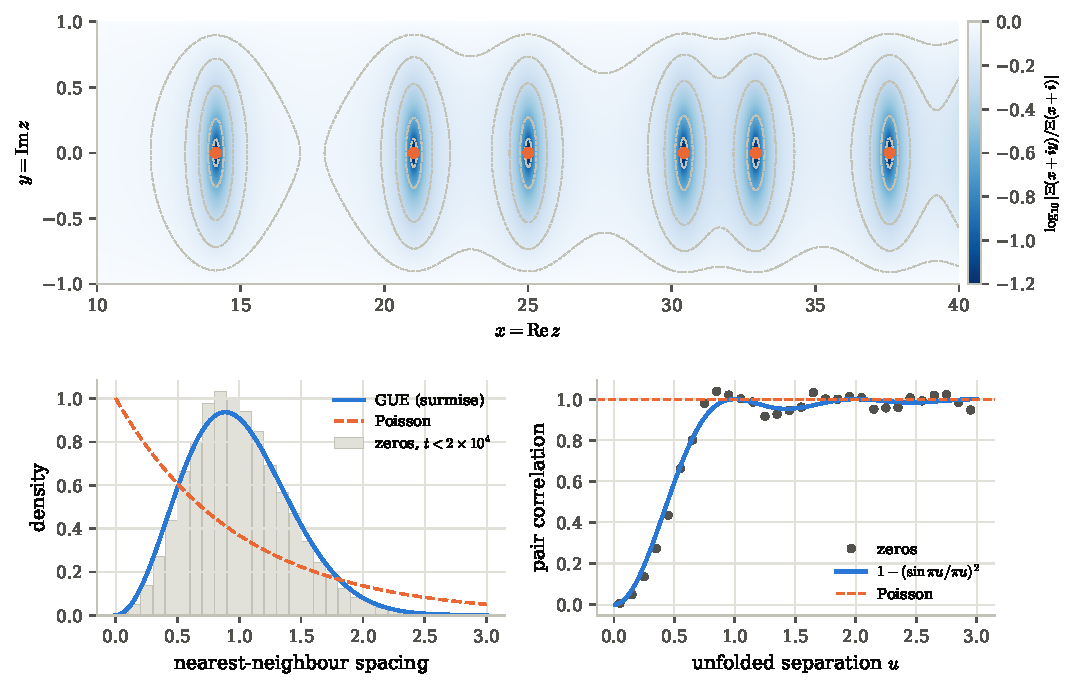
\includegraphics[width=\textwidth]{fig7_zero.pdf}
\caption{Top: the landscape $\log_{10}|\Xi(x+iy)/\Xi(x+i)|$ for $10<x<40$, $|y|<1$ (normalised at $y=1$ to remove the exponential trend); the zeros (dots) are pits on the valley floor $y=0$, and RH states that every pit lies there. Bottom left: nearest-neighbour spacings of the 22{,}491 zeros below $2\times10^4$, unfolded, against the GUE surmise and Poisson. Bottom right: their pair correlation against Montgomery's $1-(\sin\pi u/\pi u)^2$ and Poisson.}
\label{fig:zero}
\end{figure}

\section{Recurring patterns: square spirals and Euler products}\label{sec:spiral}
Recurrence in the primes is real when it has an arithmetic cause, and in the case below the cause is an Euler product. Write the integers on a square spiral with $1$ at the centre, Ulam's spiral \cite{SteinUlamWells}. The four diagonal rays are the quadratics $4k^2+4k+1$ (the odd squares), $4k^2+2k+1$, $4k^2+1$ and $4k^2-2k+1$. The Bateman--Horn conjecture \cite{BatemanHorn} (Hardy--Littlewood's Conjecture F \cite{HardyLittlewood} in this case) gives the number of primes among $f(1),\dots,f(K)$ as asymptotic to $C_f\sum_{k\le K}1/\log f(k)$ with
\[
C_f=\prod_\ell\frac{1-\omega_f(\ell)/\ell}{1-1/\ell},\qquad\omega_f(\ell)=1+\Bigl(\frac D\ell\Bigr)\quad(\ell\nmid2a),
\]
where $f(k)=ak^2+bk+c$, $D=b^2-4ac$ is the discriminant, $\omega_f(\ell)$ counts the roots of $f$ modulo $\ell$ (for odd $\ell\nmid a$, $4af(k)=(2ak+b)^2-D$, so the roots correspond to the $1+(\frac D\ell)$ square roots of $D$ modulo $\ell$), and $\omega_f(2)=0$ on every prime-bearing ray (its values are odd). For quadratic $f$ the count $C_f\sum_{k\le K}1/\log f(k)$ is asymptotic to Bateman and Horn's form $\frac{C_f}2\int_2^K du/\log u$, since $\log f(k)\sim2\log k$. The constant is an Euler product over the quadratic character $(\frac D\cdot)$, the building block of the Dirichlet $L$-functions in the Epstein zeta function of 01. For $K=2\times10^5$ the primes among $f(1),\dots,f(K)$ were counted by sieving with the roots of $f$ modulo every prime $\ell\le\sqrt{f(K)}$, and $C_f$ is the product over primes $\ell<5\times10^6$, accurate to about $10^{-4}$, which does not change the last digit of any ratio below:
\begin{center}\small
\begin{tabular}{@{}lcccc@{}}\toprule
diagonal & $D$ & $C_f$ & primes observed & observed/Bateman--Horn\\\midrule
$4k^2+4k+1$ & $0$ & --- & $0$ (reducible) & ---\\
$4k^2+2k+1$ & $-12$ & $2.241$ & $18{,}936$ & $0.9962$\\
$4k^2+1$ & $-16$ & $2.746$ & $23{,}275$ & $0.9996$\\
$4k^2-2k+1$ & $-12$ & $2.241$ & $18{,}999$ & $0.9994$\\
$k^2+k+41$ (Euler) & $-163$ & $6.640$ & $59{,}808$ & $0.9990$\\\bottomrule
\end{tabular}
\end{center}
The prime-rich and prime-poor rays of the spiral are thus read off from local factors, one per prime, exactly as the coefficients of Riemann's Wigner function are in 01 \cite{SMath}.

\section{The seven field papers, clause by clause}\label{sec:fields}
Each subsection gives the exact instance of each clause of \cref{def:instance} in one field paper, with its key theorem or number; the proofs and the computations are in the paper cited.

\subsection{01 Mathematics: the mirror, the merge and the signed current}\label{sec:f01}
\emph{The pair.} In every ring $0=s+(-s)=s(1+(-1))$, and the Dirichlet identity $\sum_{d\mid n}\mu(d)=(1+(-1))^{\omega(n)}$ is the pair sum at the level of divisors. The prime $2$ is the count at which the pair collapses (\cref{prop:parts}(c)). RH is equivalent to the balance of the two members of the sign pair, $L(x)=\sum_{n\le x}(-1)^{\Omega(n)}=O(x^{1/2+\varepsilon})$ for every $\varepsilon>0$; to $10^8$ there are $49{,}998{,}058$ integers of even length and $50{,}001{,}942$ of odd length \cite{SMath}.

\emph{The mirror and the zero.} The involution is $\iota(s)=1-s$; with conjugation it generates the Klein group $V_4$, and $\mathsf R(s)=1-\bar s$ fixes the critical line. RH holds if and only if every orbit of $V_4$ on the nontrivial zeros has size $2$. In $z=x+iy$, $H=|\Xi|^2$ is even in $y$ and the signed current $J=2\partial_yH$ is odd. A mirrored pair of zeros $\gamma\mp ib$ contributes to $J/H$
\[
\frac{8y\,(d^2+y^2-b^2)}{(d^2+(y-b)^2)(d^2+(y+b)^2)},\qquad d=x-\gamma,
\]
which is negative exactly on the half-disk $d^2+y^2<b^2$, while a real zero contributes $4y/(d^2+y^2)>0$; hence RH holds if and only if $J\ge0$ for $y>0$. 01 proves $J>0$ outside the region $\mathcal U$ of \cref{sec:intro}, from the verification of RH to height $3\cdot10^{12}$ \cite{PT} and the zero-free region with constant $5.573412$ \cite{MT}. In phase space $J=\frac14\int Q(p,x)\,p\sinh(yp)\,dp$, with $Q=8e^{p/2}\sum_N\tau_x(N)\mathcal K_x(2\pi Ne^p)$, $\tau_x(N)=N^{-ix}\sigma_{2ix}(N)$ and Mellin transform $8\,\xi(w+ix)\xi(w-ix)$; $Q(p,x)>0$ whenever $2\pi e^{|p|}\ge\max(\sqrt{2x^2+\frac12},20)$, and RH holds if and only if every even position moment of $Q$ is nonnegative at every momentum \cite{SMath}.

\emph{The triad.} In $\mathbb Z/3$ the pair $\{s,-s\}$ always occupies the positions $\frac13$ and $\frac23$; the only balanced sign function there is $\chi_{-3}$, and $L(0,\chi_{-3})=\frac23-\frac13=\frac13$. The three-state spin has its Lee--Yang zeros at $\frac13$ and $\frac23$ of a turn \cite{SMath}.

\emph{The merge.} In arithmetic the merge is the Euler product. $\xi$ is the moment function of two merged copies of one random unit, $\mathbb E[Y^s]=2\xi(s)$; one copy gives $s\pi^{-s/2}\Gamma(\frac s2)\eta(s)$, the completed alternating series of the prime two, whose zeros on $\Re s=1$ have no mirror partners; among $\nu$ merged copies the mirror holds only at $\nu=2$, and the first zero moves from $1+2\pi i/\log2$ at $\nu=1$ to $\frac12+14.134725\,i$ at $\nu=2$, the only point of its path on the critical line. The mirror without the merge leaves zeros off the line: the Davenport--Heilbronn function has four mirrored pairs off the line below height $200$, while all $114$ zeros of $L(s,\chi_{-3})$ there lie on it; and an Epstein zeta function with the functional equation and no Euler product has a kernel with an expansion and a tail theorem of the same form as those of $\Phi$, and a current that is negative near its off-line zero. Every proof of $J\ge0$ must therefore use the Euler product \cite{SMath}.

\emph{The fourth.} Two merged elementary pairs have four configurations and three values of their sum, and the fourth configuration lands on the zero of the triad (\cref{prop:merge,prop:fourth}). On the zeros of $\xi$ the mirror and conjugation generate a group of order four, and RH says that every orbit uses only half of it.

\emph{The 2026 proportion.} Known unconditional results carry the balance part of the way (\cref{tab:prior}). The proportion of zeros proved to lie on the critical line first passed one third \cite{Levinson}, exceeds five twelfths in published work \cite{PRZZ}, and exceeds two thirds in a preprint of August 2026, which proves that a proportion at least $0.6725$ of the zeros, counted with multiplicity, are simple and lie on the line \cite{AF}; 01 records these results beside its own \cite{SMath}.

\subsection{02 Physics: the reversible half and the third body}\label{sec:f02}
\emph{The pair and its zero.} Time reversal maps a record chain $C$ with stationary law $\pi$ to $\tilde C=D_\pi C^{\mathsf T}D_\pi^{-1}$, and $C=S+A$ splits into the reversible half $S=\frac12(C+\tilde C)$, which satisfies detailed balance, and the irreversible half $A=\frac12(C-\tilde C)$. The zero is detailed balance, $J=J^{\mathsf T}$. 02 proves
\[
h(S)-h(C)=\sum_j\pi_j\,\mathrm{JSD}(C_{\cdot j},\tilde C_{\cdot j}),\qquad 0\le h(S)-h(C)\le\tfrac14\,\mathrm{EP},
\]
with equality to leading order as $A\to0$, from the pointwise inequality $\mathrm{JSD}\le\frac18\times$(Jeffreys divergence). For a processed four-outcome instrument $\mathrm{EP}=0.00686044$ bits per use and $h(S)-h(C)$ reaches $99.86\%$ of $\mathrm{EP}/4$; for alternating sharp measurement of a singlet the stationary record is reversible and the whole arrow, $c\,\mathrm{artanh}(c)$ nats with $c=\cos\frac\pi n$, is the Jeffreys divergence of the seed pair law from the stationary one \cite{SPhys}. In the three-phase field the symmetric half of the lagged correlation carries the magnitude $|I_+|^2+|I_-|^2$ and the antisymmetric half the signed swept area $\frac{9\pi}4(|I_+|^2-|I_-|^2)$.

\emph{The triad.} For three equal masses with the centre of mass at the origin, every collinear instant with one body at the midpoint is the triad $(-s,0,s)$. The figure-eight has period $T=6.3259140121$, is a choreography to $4.1\times10^{-12}$, holds the triad six times per period at $kT/6$ to $5.5\times10^{-9}$ with each body at the zero twice, and carries no harmonic divisible by three, by $1+u+u^2=0$ (to $7.2\times10^{-13}$); its time-reversal symmetry makes its angular momentum vanish harmonic by harmonic, a balance of counter-rotating pairs \cite{SPhys}.

\emph{The merge.} Gravity couples every pair of bodies with the same sign. The triad with a body at the zero keeps its shape within $3.2\times10^{-6}$ over $50$ periods after a $10^{-6}$ kick, while the equal-mass Lagrange triangle, with no body at the zero, grows at $0.702194$ against the exact $\omega/\sqrt2=0.702331$; a triangle of general masses stands only around a dominant centre, $m_1>0.9614791\,M$ \cite{SPhys}.

\emph{The fourth.} A fourth body of mass $\varepsilon$ at distance $D$ outside the Mardling--Aarseth boundary forms a new pair with the triad, $3X_{\mathrm{triad}}+\varepsilon x_4=0$; it lends the triad a spin and takes it back every half outer orbit, deforming it by
\[
\delta_{\max}\simeq\sqrt3\,\langle\Delta I\rangle\,\varepsilon D^{-3/2}=2.84\,\varepsilon D^{-3/2};
\]
inside the boundary it is expelled. The singlet, the fourth state of $\frac12\otimes\frac12=1\oplus0$, writes a reversible stationary record \cite{SPhys}.

\subsection{03 Quantum: the Riemann kernel as a quantum state}\label{sec:f03}
\emph{The pair and its zero.} $\Phi$ is even, so $\varphi=\Phi/\|\Phi\|$ is a parity eigenstate and its momentum wave function $\Xi$ is even and real on $\R$; its zeros come in sets $\{z,-z,\bar z,-\bar z\}$, and the fixed line of $z\mapsto\bar z$ is the real axis. For the observables $\hat O_{x,y}$ with nonnegative Weyl symbol $a\sinh(2ya)\,\delta(k-x)$, 03 proves
\[
\langle\psi|\hat O_{x,y}|\psi\rangle=\tfrac12\,\partial_y|\tilde\psi(x+iy)|^2
\]
for every real even or odd state of sufficient decay, so the family detects every state whose momentum wave function has a non-real zero and no state whose momentum wave function has order at most one and only real zeros, and RH holds if and only if $\varphi$ is not detected; $J=2\pi\|\Phi\|^2\langle\varphi|\hat O_{x,y}|\varphi\rangle$. The Wigner negativity of $\varphi$ carries $4.844\times10^{-5}$ of the mass and is confined, at every momentum, to $2\pi e^{2|a|}<\max(\sqrt{2k^2+\frac12},20)$ \cite{SQuant}.

\emph{The coherence equivalence.} A qubit dephased by a classical field with law $\Phi/\int\Phi$ has coherence $L(t)=\Xi(\lambda t)/\Xi(0)$, and RH holds if and only if $L$, continued to complex time, vanishes only at real times; under RH every local minimum of $|L|$ is a zero. The coherence vanishes at the first five ordinates to $1.0\times10^{-9}$, and a bath of $64$ classical levels reproduces $\gamma_1,\gamma_2,\gamma_3$ to $7.1\times10^{-10}$. Along the de Bruijn--Newman flow, detection of the filtered state, complex-time zeros of the filtered probe and $T<\Lambda$ are one condition, and RH is $\Lambda=0$ \cite{SQuant}.

\emph{The triad.} A maximally mixed spin-1 gives $L=(1+2\cos2\lambda t)/3$ and complete decoherence at exactly $\frac13$ and $\frac23$ of the revival period (\cref{prop:fourth}(b)).

\emph{The merge.} The spin-1 is the merged pair of two Ising spin-$\frac12$'s at coupling $\frac12\ln2$ (\cref{prop:merge}(c)). Every chain of $N$ triads with coupling $K\ge0$ decoheres completely at $2N$ real times per period, counted with multiplicity, and has no partial dips; for $N=2,\dots,6$ at four couplings all roots lie on the circle to $8.2\times10^{-14}$. At $K=-1$ roots leave the circle (to $|z|=13.9393$), and even chains never decohere fully ($|L|\ge0.05311$) \cite{SQuant}: the Lee--Yang zeros under positive coupling stay on the circle, and under negative coupling they leave it.

\emph{The fourth.} The probe qubit is the observer, and the singlet is the fourth state of the merged pair, which turns the thirds into $1{:}2{:}1$ and $\cos^2\lambda t$ (\cref{prop:fourth}(c)). 03 proposes an NMR realisation: a ${}^{13}$C probe bonded to one deuteron, whose coherence $(1+2\cos2\pi\mathcal Jt)/3$ vanishes at $t=1/3\mathcal J$ and $2/3\mathcal J$; a CD$_3$ group with threefold zeros at the thirds; a pair of triads with $K=1$, which decoheres completely at $\mathcal Jt=0.179649$, $0.396437$, $0.603563$, $0.820351$, and with $K=-1$ never ($|L|\ge0.2839$); and a weighted Ramsey sequence that realises the $64$-level Riemann bath \cite{SQuant}.

\subsection{04 Chemistry: which member carries}\label{sec:f04}
\emph{The pair.} The weights of a two-state pair are $\frac12\pm\delta$ with $\delta=-\frac12\tanh(\varepsilon/2)$, and an observation of which member holds something determines $\delta$ (\cref{prop:twostate}). One electron and two cores: with $\Delta E=\mathrm{IE(Na)}-\mathrm{IE(K)}=0.7984132(3)$ eV, potassium carries the charge, and the minority configuration $\mathrm{Na^+}+\mathrm K$ of the separated pair has occupancy $3.87\times10^{-14}$ at $300$ K, while in an equimolar gas mass action gives the converted fraction $x$ by $x/(1-x)=e^{-\Delta E/2k_BT}$, that is $x=1.97\times10^{-7}$: the exponent is halved because the two products form independently. For ${}^{40}$K the net charge change per decay is twice the odd part, $\langle\Delta Z\rangle=2p_{\beta^-}-1=2\delta$ with $p=p_{\beta^-}$: $+0.7856(22)$ from the 2017 ENSDF evaluation and $+0.7918(10)$ from the 2023 KDK branching ratios, $2.6$ combined standard uncertainties apart. For aluminium's ground term the upper fine-structure level is the majority above $T_{1/2}=232.61$ K, and tends to $\frac23$, the pair at $\varepsilon=-\ln2$ (\cref{prop:twostate}(d)) \cite{SChem}.

\emph{The common part is decisive in a shared code.} If a fraction $f$ of rows is absent in two channels and filled with codes at standardised distances $d_x,d_y$ from the present-row means, the correlation becomes exactly $(r+fd_xd_y)/\sqrt{(1+fd_x^2)(1+fd_y^2)}$; its sign flips when $\sqrt{d_xd_y}$ crosses $\sqrt{-r/f}$. For two sensor channels of the UCI air-quality record \cite{UCIair} ($r=-0.771918$, $f=366/9357$) the flip lies at $4.4424$; computed from the workbook, the codes $-200$ and $0$ sit at $\sqrt{d_xd_y}=4.9133$ and $4.0595$, and the closed form reproduces the coded correlations $+0.0869312$ and $-0.0756296$ to within $10^{-16}$ \cite{SChem}.

\emph{The sensor ladder, with S3 as the opposite member.} Mass action makes the ionosorbed-oxygen occupancy of a metal-oxide surface an exact logistic, $\theta=1/(1+\e^{\varepsilon})$ with $\varepsilon=\ln(\Phi_+/\Phi_-)$ the log-ratio of the electron-release and trapping flux coefficients; under three stated approximations $\varepsilon$ is linear in $\beta_R\ln C_R-\beta_O\ln C_O$. On the common CO axis of the air record the two-state law beats the offset power law for every sensor ($\Delta$AIC $11.7$ to $209.0$) and identifies the half-points $C_{1/2}=1.68$ mg\,m$^{-3}$ for the tungsten-oxide sensor S3 ($95\%$ interval $[1.39,1.98]$), $4.61$ for S5 and $5.40$ for S2, with S1 at $7.49$ at the upper edge of the data, with slopes $\beta=1.18$--$1.45$ just above first order; the order S3 $<$ S5 $<$ S2 holds in both halves of the year. S1, S2, S4 and S5 rise with every traffic gas and S3 falls with every one: S3 is the opposite member of the ladder, the same law with $S_{\mathrm{hi}}<S_{\mathrm{lo}}$. The benzene column of the record is an exact power-law transform of S2, $1.23978\times10^{-4}(S_2-324.785)^{1.743158}$ to $1.6\times10^{-15}$ relative. NO$_2$ is co-emitted with the reducing gases, so with NO$_2$ as the oxidizing marker the pair regression gives same-signed coefficients; the one robust opposite-sign competition in the record is CO against NO on S4, with balance slope $3.28$ $[2.90,3.73]$ \cite{SChem}.

\emph{Döbereiner's triads.} Every orbital holds a spin pair, and the Madelung order gives the period-pair law $L(p)=2\lceil(p+1)/2\rceil^2$, that is $2,8,8,18,18,32,32$. A vertical triad $Z_1<Z_2<Z_3$ is exact, $Z_2=\frac12(Z_1+Z_3)$, if and only if the two periods it spans have equal length; $27$ of the $54$ vertical triads are exact, with common gap $s=8$ ($3$ triads), $18$ ($8$) or $32$ ($16$), and Döbereiner's four are among them. The middle element is the zero of the pair $(-s,+s)$, and the triad is $Z_2+\{-s,0,s\}$ \cite{SChem}.

\emph{The merge and the fourth.} Exact triads in one group meet end to end: K ends Li--Na--K and begins K--Rb--Cs. The shared end is the observer of the first triad and a member of the next, and the chain is the merge of triads along a group \cite{SChem}. The two-state law of the sensor is the law of the gates of 05 and of the NH$_4$SH deck of 07 (\cref{sec:together}).

\subsection{05 Neuroscience: the gate, the balanced cortex and the 3+1 channel}\label{sec:f05}
\emph{The gate.} A voltage-gated channel's gate has two states and open occupancy $p(V)=1/(1+e^{-z(V-V_{1/2})})$. The half-point is the zero of the pair: there the occupancy is $\frac12$, the entropy one bit and the variance largest, and the occupancies $\frac13$, $\frac23$ lie at $V_{1/2}\mp k\ln2$. The Hodgkin--Huxley half-points are $-40.02$ ($m$), $-62.31$ ($h$) and $-53.41$ mV ($n$). A membrane reading determines what the pair lets it: mean currents fix only the product $Ni$ of channel number and unitary current, and the variance separates them; a spike threshold fixes $V_a$ and $g_{\mathrm{Na}}$ only through $g_{\mathrm{Na}}e^{-V_a/k_a}$ \cite{SNeuro}.

\emph{The merge.} Adding independent identical gates keeps the pair: the normalised mean current is $p(V)$ with the half-point of one gate. Multiplying gates does not: $n_\infty^4$ crosses $\frac12$ at $-18.88$ mV, $34.5$ mV above the half-point of its gate \cite{SNeuro}.

\emph{The balanced E--I zero.} Every row of the connectivity of the balanced network is ternary, $\{+1,0,-J_X\}/\sqrt K$. 05 proves that the residual net input and the distance of the rates from the balance solution are one object,
\[
\mu=\sqrt K\,A\,(\nu-\nu_{\mathrm{bal}}),\qquad \nu-\nu_{\mathrm{bal}}=A^{-1}\mu/\sqrt K,
\]
with $A$ the matrix of the balance equations. In simulations of $2\times10^4$ binary neurons with $K=100$ to $1600$ the identity reproduces the measured rates to $2.67\times10^{-3}$; excitation and inhibition grow as $\sqrt K$ per unit rate (log--log slopes $0.4994$--$0.5004$; the components themselves have slopes $1.096$ and $0.677$, because the rates are still rising), the net input stays of order one, and fractions $0.9763$ (E) and $0.9954$ (I) of the excitatory drive cancel at $K=1600$. The rates approach the balance solution slowly, $40.6\%$ (E) and $22.2\%$ (I) below it at $K=1600$, exactly as the identity requires: $\det A=0.2$ amplifies the residual, and mean-field rates come within $10\%$ of balance for $K>40{,}054$ (E) and $K>8{,}897$ (I) \cite{SNeuro}.

\emph{The 3+1 sodium channel.} The sodium conductance $m^3h$ is a triad with a fourth: three activating particles, like the channel's three fast voltage sensors in domains I--III, and one inactivating particle, like the domain IV sensor, which alone is sufficient and rate limiting for fast inactivation. Its spike (amplitude $104.06$ mV) carries $13.36$ times the minimum sodium charge, its inward and outward charges cancel exactly, and among exponents $1$ to $4$ only $m^3h$ gives both a stable rest and a spike. The sodium--potassium pump is the unequal pair $3{:}2$, with common part $\frac52$ and half-difference $\pm\frac12$, and moves one elementary charge per cycle \cite{SNeuro}.

\subsection{06 Algorithms: the triad as a digit set}\label{sec:f06}
\emph{The triad digit set.} Balanced ternary writes every integer with digits in $\{-1,0,1\}$, the triad of \cref{prop:triad}. Every integer has exactly one representation; negation $\iota(n)=-n$ is the digit flip, with fixed set $\{0\}$; in $n=\operatorname{sgn}(n)\,|n|$ the factor odd under $\iota$, the sign, is the leading nonzero trit, and the even factor $|n|$ carries the magnitude; the carries of addition stay in the triad, products of digits need no carry, rounding is truncation (with its exact tie case at the half-integers), and order is lexicographic. A width-$d$ register holds $0$ and exactly $(3^d-1)/2$ pairs $\{m,-m\}$. Exhaustive enumeration over all $|n|\le3^{10}$, and over all $|a|,|b|\le3^5$ for the addition rule, agrees with every one of these statements \cite{SAlg}.

\emph{Radix 3 is the cheapest.} Writing $0,\dots,N$ in base $b$ costs $C_b(N)=b\,d_b(N)$ digit-states. Its growth rate $E(b)=b/\ln b$ is minimised among integers uniquely at $b=3$, with $E(2)/E(3)=E(4)/E(3)=\frac23\log_23=1.0566$; base $3$ is a cheapest base for every $N\ge2^{16}$ and the unique cheapest base for every $N\ge2^{27}$, and both thresholds are sharp \cite{SAlg}.

\emph{The merge.} The generating function of a width-$d$ register is the product of one factor per trit,
\[
Z_d(z)=\prod_{i=0}^{d-1}\bigl(z^{-3^i}+1+z^{3^i}\bigr)=\sum_{|n|\le(3^d-1)/2}z^n ,
\]
and vanishes exactly at the $3^d-1$ nontrivial $3^d$-th roots of unity, all on the unit circle: merging digits with the positive weights $3^i$ keeps every zero on the circle and fills it at the $3^d$-ths of a turn \cite{SAlg}.

\emph{The fourth.} A comparator reads two registers and returns $\operatorname{sgn}(a-b)\in\{-1,0,1\}$, a digit of the same triad; a probe reading a uniformly distributed register has $L(t)=\sin(3^d\lambda t)/(3^d\sin\lambda t)$, which for $d=1$ is \cref{prop:fourth}(b). The least-squares ternary quantiser has threshold $\Delta=\alpha/2$ and, for uniformly distributed weights, sets exactly one third of them to zero; no odd quantiser onto $\{-\alpha,\alpha\}$ exists, since an odd map into an alphabet $A=-A$ must send $0$ to $0\in A$. A $64$--$128$--$10$ network with weights in $\{-\alpha,0,+\alpha\}$ reaches $97.44\pm0.73\%$ on the UCI handwritten digits \cite{UCIdigits}, against $97.70\pm0.43\%$ with 32-bit floats and $97.11\pm0.55\%$ with binary weights, at $\log_23=1.585$ bits per weight \cite{SAlg}.

\subsection{07 Planetary science: throats, the gas ladder and the four giants}\label{sec:f07}
\emph{The pair: two throats about one centre.} Every giant's Hill sphere opens through two throats, at $L_1$ and $L_2$, a pair about the planet. Their linear dynamics is the same for every planet: the collinear points of Hill's problem have
\[
\lambda^4-2\lambda^2-27=0,\qquad \lambda_H=\sqrt{1+2\sqrt7}=2.508287,\quad \omega_H=\sqrt{2\sqrt7-1}=2.071594,
\]
so $\lambda_H^2-\omega_H^2=2$ and $\lambda_H^2\omega_H^2=27$, with vertical frequency $2$. 07 proves that the pair is unequal by $\mathcal A=\frac h3(1-\frac{h^2}{27}+O(h^3))$, $h=(\mu/3)^{1/3}$, and confirms it in the full problem ($0.99972$, $0.99989$, $0.99997$ and $0.99997$ of $h/3$ for Jupiter, Saturn, Uranus and Neptune). The transmission through a throat is the two-state law, $T=1/(1+\e^{-2\pi\Delta E/\hbar\lambda})$, balanced at the saddle energy \cite{SPlanet}.

\emph{The zero: the NH$_4$SH titration.} Where NH$_4$SH(s) coexists with the gas, $x_{\mathrm{NH_3}}x_{\mathrm{H_2S}}=k^2=K(T)/P_{\mathrm{atm}}^2$, and the solid takes the two gases one for one. With $x_{\mathrm{NH_3}}=k\e^{\varepsilon/2}$ and $x_{\mathrm{H_2S}}=k\e^{-\varepsilon/2}$ the common part is the geometric mean $k$, and the odd part $\Delta=\mathrm N-\mathrm S=2k\sinh(\varepsilon/2)$ is conserved; as $k\to0$ above the deck, the surviving member is $\mathrm{sign}(\mathrm N-\mathrm S)$, and at $\mathrm N=\mathrm S$ neither survives. The zero at $\mathrm N/\mathrm S=1$ decides the top deck: on every planet's profile the top ice is H$_2$S for every $\mathrm N/\mathrm S<1$, NH$_3$ for every $\mathrm N/\mathrm S>1$, and neither at $\mathrm N/\mathrm S=1.000$. With deep $\mathrm N/\mathrm S=4.73$, $3.16$, $0.195$ and $0.170$ for Jupiter, Saturn, Uranus and Neptune, this is why the ice giants show H$_2$S and not NH$_3$ above their clouds; the model's saturated H$_2$S at the cloud tops, $0.26$--$1.8$ ppm on Uranus and $0.49$--$2.25$ ppm on Neptune, brackets the detected $0.4$--$0.8$ ppm on Uranus and overlaps the detected $1$--$3$ ppm on Neptune \cite{SPlanet}.

\emph{The rungs.} An equilibrium cloud-condensation model anchored at the $1$-bar temperatures gives $3,3,4,4$ decks: NH$_3$ ice, NH$_4$SH and H$_2$O at $0.763$, $2.380$ and $5.832$ bar on Jupiter and $1.537$, $5.130$ and $14.68$ bar on Saturn; CH$_4$ ice, H$_2$S ice, NH$_4$SH and H$_2$O at $1.364$, $6.263$, $34.98$ and $200.5$ bar on Uranus and $1.619$, $6.973$, $37.59$ and $224.5$ bar on Neptune. Each deck base is a half-point, where the log saturation ratio vanishes. Jupiter and Saturn carry the triad of decks and the ice giants a fourth, methane, on top; the count is the same in all $179$ abundance-range cases \cite{SPlanet}.

\emph{The triad and the Krein collision.} The triangular points are a triad with a centre, stable by the Gascheau--Routh criterion $27\sum_{i<j}m_im_j<M^2$. At $L_4$ the characteristic polynomial is $\lambda^4+\lambda^2+\frac{27}4\mu(1-\mu)=0$; below $\mu_G=0.0385209$ the spectrum lies on the imaginary axis in two pairs of opposite Krein signature, which leave it only by colliding: they meet at $\omega=1/\sqrt2$ exactly at $\mu_G$, and at $\mu_G(1+10^{-4})$ the four are $\pm0.00346\pm0.70712\,i$, a mirrored quadruple. Io, Europa and Ganymede form a locked triad, $n_{\mathrm{Io}}-3n_{\mathrm{Eu}}+2n_{\mathrm{Ga}}=-0.000029$ deg/day, with Callisto outside at a period ratio of $2.33264$; Jupiter and Saturn meet two thirds of a turn apart, and the triangle of their conjunctions turns one third of a turn in exactly one period of the great inequality, $883$ years \cite{SPlanet}.

\emph{The fourth: three live modes and one zero mode.} To first order in the masses the inclinations of the four orbits evolve under a Laplace--Lagrange matrix whose rows sum to zero, so a common tilt is an exact zero mode: the invariable plane, occupied by no body. The three live modes have frequencies $-25.5183$, $-2.9276$ and $-0.6698$ arcsec/yr. Four is three and a zero \cite{SPlanet}. The rest of the planetary system is the fourth body that depletes the Trojans of the stable triangles; three equal vortices with an equal fourth at the centre sit exactly on the edge of stability; the interstellar objects 1I, 2I and 3I share neither a direction nor a kinematic origin (largest pairwise velocity difference $75.5$ km/s); and 3I/ATLAS touched Jupiter's Hill sphere at $1.0011$ Hill radii. 3I/ATLAS was not the source of the Wow!\ signal: in 1977 it lay $8.3^\circ$ from the nearer beam centre of the Big Ear telescope, and a hydrogen-line transmitter on it would have been received $11.6$ channels away from the Wow!\ signal \cite{SPlanet}.

\section{Five identities across the set}\label{sec:together}
The field papers share more than a language. The following five statements are identities: each holds with the same formula in every paper cited.

\paragraph{(I) One two-state law.} The occupancy $p=1/(1+\e^\varepsilon)$ with even part $\frac12$ and odd part $\delta=-\frac12\tanh(\varepsilon/2)$ (\cref{prop:twostate}) is the open occupancy of a gate with $\varepsilon=-z(V-V_{1/2})$ (05); the occupancy of an atomic level with $\varepsilon=\Delta E/k_BT-\ln(g_u/g_l)$ and of a surface site with $\varepsilon=\ln(\Phi_+/\Phi_-)$ (04); the H$_2$S share of the vapour above the NH$_4$SH deck with $\varepsilon=\ln(x_{\mathrm{NH_3}}/x_{\mathrm{H_2S}})$ and the transmission through a throat with $\varepsilon=-2\pi\Delta E/\hbar\lambda$ (07). In each the occupancy depends on $\varepsilon$ alone, so what is common to the two members cancels from the observable; on the sensor this is a factor common to $\Phi_\pm$, in the deck the geometric mean $k$. In each the observer reads the odd part only: which member holds the electron, which gas survives the deck, the net charge change of a decay. The occupancies $\frac13$ and $\frac23$ are the pair $\varepsilon=\pm\ln2$: the gate at $V_{1/2}\mp k\ln2$ (05), the high-temperature limit $\frac23$ of aluminium's doublet (04), and the uniform triad, in which the zero holds $\frac13$ and the pair $\frac23$, reached by the merge at coupling $\frac12\ln2$ (01, 03).

\paragraph{(II) One triad generating function.} $z^{-1}+1+z$ is the Lee--Yang polynomial of the three-state spin (01), three times the coherence of a probe reading a spin-1 (03), the generating function of one trit (06), and, through $1+u+u^2=0$, the identity that removes the harmonics divisible by three from a three-body choreography and the zero-sequence current from a three-phase field (02). Its zeros at $\frac13$ and $\frac23$ of a turn are the thirds of the principle. The same value $\frac13$ is $L(0,\chi_{-3})=\frac23-\frac13$ in arithmetic (01) and the zero share of the least-squares ternary quantiser for uniform weights in quantisation (06).

\paragraph{(III) One merge rule.} A positive merge keeps zeros on the fixed set; a negative or absent merge lets them leave it in mirrored pairs. Positive: ferromagnetic chains of triads (01, 03), the Euler product (01), a register with weights $3^i$ (06), sums of independent gates (05). Negative or absent: antiferromagnetic chains, whose zeros leave the circle in pairs $z,1/\bar z$ (01, 03); the Davenport--Heilbronn function and the Epstein zeta function, with the mirror and without the Euler product (01); products of gates, which move the half-point (05).

\paragraph{(IV) One Klein group.} Let an involution $\iota$ of $\C$ and complex conjugation generate a Klein four-group $V$ acting on a set of zeros or eigenvalues. A generic orbit has four elements, $\{w,\iota w,\bar w,\iota\bar w\}$; on the fixed set of the composition $w\mapsto\iota\bar w$ it collapses to the pair $\{w,\iota w\}$. For the zeros of $\xi$, $\iota(s)=1-s$ and the fixed set is the critical line: RH states that every nontrivial zero lies there (01). For the spectrum of a real linear Hamiltonian system, $\iota(\lambda)=-\lambda$ and the fixed set is the imaginary axis: the Gascheau--Routh criterion states when every eigenvalue at $L_4$ lies there, and Krein's theorem states that eigenvalues leave it only when two pairs of opposite signature collide, as a quadruple (07). For the Lee--Yang zeros of a real partition function with $Z(1/z)=Z(z)$, $\iota(z)=1/z$ and the fixed set is the unit circle: the Lee--Yang theorem states that every zero of a ferromagnet lies there, and an antiferromagnetic coupling sends zeros off it as pairs $z,1/\bar z$ (01, 03). In all three, a zero on the fixed set is its own mirror image under $w\mapsto\iota\bar w$.

\paragraph{(V) One observer.} The probe coherence $L(t)=Z(\e^{-2i\lambda t})/Z(1)$ (\cref{prop:fourth}(d)) makes the complete-decoherence times of a probe the Lee--Yang zeros of what it reads (03), the zeros of $\Xi$ for Riemann's spin (03, readings 3 and 7), the thirds for a triad (03) and the $3^d$-ths for a register (06). The observer's record is balanced: the phases at complete decoherence are roots of unity summing to zero; the comparator's output is a trit (06); the fourth body forms with the triad a new pair about their joint centre (02); a neuron's output enters other neurons' ternary rows (05).

\section{The Riemann Hypothesis in the set}\label{sec:rh}
By the pair formula and the unconditional region (\cref{sec:f01}), \cref{conj:RH} is equivalent to $J\ge0$ on $\mathcal U$. 01 states this remaining step as a conjecture \cite{SMath}.

\begin{conjecture}\label{conj:step}
For every $x$ with $|x|>3\cdot10^{12}-\frac12$ and every $0<y<\frac12-1/(5.573412\log(|x|+\frac12))$, the Euler-product-weighted sum of Macdonald functions $\int_\R Q(p,x)\,p\sinh(yp)\,dp$ is positive.
\end{conjecture}

\Cref{conj:step} is equivalent to \cref{conj:RH}: if RH holds, every term of the pair formula is positive and $H>0$ for $y>0$, so $J>0$; conversely, \cref{conj:step} and $J>0$ outside $\mathcal U$ give $J\ge0$ for all $y>0$. The set proves that \cref{conj:RH} is equivalent to each of the following:
\begin{enumerate}[label=(\alph*)]
\item every even position moment of Riemann's Wigner function is nonnegative at every momentum (01, 03);
\item the margin of the ledger is nonnegative on $\mathcal U$, $A\le G$ (01);
\item the sign pair is balanced, $M(x),L(x)=O(x^{1/2+\varepsilon})$ for every $\varepsilon>0$ (01);
\item every orbit of the mirror group $V_4$ on the nontrivial zeros has size two (01);
\item the Riemann spin has the Lee--Yang property: $\int\Phi(\tau)e^{h\tau}d\tau$ vanishes only for imaginary $h$ (01; reading~3 of \cref{sec:zero});
\item $\Lambda=0$ for the de Bruijn--Newman constant, and the coherence of a probe dephased by a field with law $\Phi/\int\Phi$, continued to complex time, vanishes only at real times (03).
\end{enumerate}

\paragraph{What the set fixes about the remaining step.} Kernel positivity alone reaches $y\gtrsim5.24x$. Near the line the sign is decided in the oscillatory head, at $x=50$ in the Airy transition zone. And a proof must use a property that $\zeta$ has and the Epstein zeta function lacks, such as the Euler product: positivity, evenness, decay, the theta-series origin, the expansion and the tail theorem are shared by the Epstein kernel, whose current is negative near its off-line zero (01).

\begin{remark}[three sufficient conditions]\label{rem:routes}
Each of the following implies \cref{conj:RH}, and each is stated in the terms of the set. (i) A representation of $J/H$ for $y>0$ as a relative entropy between two probability laws, which is nonnegative for the same reason as the entropy production $\mathrm{EP}$ of a record chain, itself a relative entropy (02); it would make RH a second law in that sense. (ii) A proof that $\Phi$ lies in the Griffiths--Simon class of limits of positively merged elementary pairs \cite{SimonGriffiths}, which with the Lee--Yang theorem gives RH as the merge clause (01, 03). (iii) A self-adjoint operator with the zeros as eigenvalues, which gives RH as spectral reality (reading~5 of \cref{sec:zero}).
\end{remark}

\section{Concluding remarks}\label{sec:concl}
We have stated the Triad Principle as one involution and proved its five clauses (\cref{thm:principle}); given the exact instance of every clause in each of the seven field papers (\cref{tab:master}); and shown that five structures recur across them as identities. For $\xi$ the involution is the functional equation; it comes from Poisson summation, as T-duality does, and its zeros are, in seven readings, balances of two equal halves of the kernel mass, vortices of the phase, Lee--Yang zeros, resonances, spectral levels, masses and transition times. In the set, the Riemann Hypothesis is equivalent to seven statements and reduces to \cref{conj:step}, whose proof must use the merge.

\paragraph{Outlook.} The routes of \cref{rem:routes} state the remaining step for the Riemann Hypothesis in the language of entropy, of merged spins and of spectra. The thirds and the balance are ready for direct measurement: a ${}^{13}$C probe bonded to one deuteron decoheres completely at $t=1/3\mathcal J$ and $2/3\mathcal J$ (03), balanced networks beyond $K=40{,}054$ (E) and $8{,}897$ (I) reach the regime in which mean field places the rates within $10\%$ of balance (05), and an oxidizing marker that is not co-emitted with traffic, with an ozone reference for S5, will separate the two members of the sensor pair (04). For the giants, a deep survey of the annulus $42$--$51$ million km from Uranus ($0.60$--$0.73$ of its Hill radius), a long continuous record of Saturn's disk or gravity at the acoustic spacing of $112$--$117\,\mu$Hz computed in 07, a deep N/S for Neptune, O/H, and the ortho/para state of hydrogen will fix the remaining rungs of the ladder \cite{SPlanet}.

\section{Data and sources}\label{sec:data}
No measured data and no physical constants enter the computations of this paper. Every number in \cref{sec:poisson,sec:eis,sec:zero,sec:spiral} is computed, in double-precision arithmetic, from the formulas and by the methods stated where it appears: Gauss--Legendre and trapezoidal quadrature, Euler--Maclaurin summation of $\zeta$, the Riemann--Siegel formula, the argument principle and sieving. Numbers quoted from the field papers are computed there by the methods each paper states. The external inputs are the following.
\begin{itemize}
\item \emph{Zeros of $\zeta$.} $\gamma_1=14.134725141734693790$, $\gamma_2=21.022039638771554993$, $\gamma_3=25.010857580145688763$ (reading~1; $\gamma_1,\gamma_2$ in reading~2; $\rho_1=\frac12+i\gamma_1$ in reading~4) and $\gamma_4=30.424876125859513210$, $\gamma_5=32.935061587739189691$, $\gamma_6=37.586178158825671257$ (the dots in \cref{fig:zero}), rounded to 18 decimals from Odlyzko's table of the first 100 zeros \cite{OdlyzkoTables}. We re-located each one as a root of $Z(t)$, with $\zeta(\frac12+it)$ computed by Euler--Maclaurin summation; the roots agree with the table to $10^{-14}$, and $|\Xi(\gamma_n)|<2\times10^{-17}$ with $\Xi$ computed from the kernel. The first five, to six decimals, also served to check the accuracy of the zeros computed in reading~5.
\item \emph{Lehmer's pair}, the zeros at $t\approx7005.0627$ and $t\approx7005.1006$ \cite{Lehmer}, used only to identify the closest pair found in reading~5.
\item \emph{The 22{,}491 zeros of reading~5} are computed here as described there. They are the only data set of this paper's own computations, and the lower panels of \cref{fig:zero} are drawn from them. The upper panel is $\Xi$ computed from the kernel on a $601\times101$ grid of $10\le x\le40$, $|y|\le1$.
\item \emph{Constants.} $\Xi(0)=\xi(\frac12)=-\frac18\pi^{-1/4}\Gamma(\frac14)\zeta(\frac12)=0.4971207782$, with $\zeta(\frac12)=-1.4603545088$ by Euler--Maclaurin summation; the kernel integral $\int_0^\infty\Phi$ reproduces this value to $10^{-13}$. $\zeta(2)=\pi^2/6$; $\zeta(3)$ and all other values of $\zeta$ by Euler--Maclaurin summation.
\item \emph{The Epstein example} (the form $2m^2+3n^2$, its kernel and zeta function) is that of 01 \cite{SMath}; its off-line zero quoted in reading~3 was located here by Newton's method applied to $\xi_\epsilon(\frac12+iz)$.
\item \emph{Results quoted from the literature without recomputation}: the amplitude of \cite{Remmen} (reading~6) and the experiment of \cite{Wei} (reading~7); the verification of RH to height $3\cdot10^{12}$ \cite{PT}; the zero-free region $\beta<1-1/(5.573412\log|\gamma|)$ \cite{MT}; the critical-line proportions: more than one third \cite{Levinson}, more than five twelfths \cite{PRZZ}, and at least $0.6725$ simple and on the line \cite{AF}. No number from them enters a computation here.
\item \emph{Results quoted from the field papers.} Every number of \cref{tab:master} and of \cref{sec:fields,sec:together,sec:rh,sec:concl} is taken from the paper cited, whose Data and sources section lists its external inputs with values and sources. The data sets behind them are: the transition matrix of a processed four-outcome instrument and the figure-eight initial data of Sim\'o as published by Chenciner and Montgomery (02); the NIST Atomic Spectra Database, the ENSDF and KDK evaluations of ${}^{40}$K, the CIAAW standard atomic weights, and the UCI Air Quality data set \cite{UCIair}, hourly responses of five metal-oxide sensors with reference-analyser concentrations recorded in an Italian city from March 2004 to April 2005, of which all $9357$ dated rows of the workbook were used (04); the Hodgkin--Huxley rate functions and squid-axon parameters (05); the UCI Optical Recognition of Handwritten Digits data set \cite{UCIdigits}, of which the $1797$ images of the test partition were used (06); and the NASA NSSDC planetary fact sheets, published abundances, gravity fields and thermodynamic data, the moon lists, the orbital elements of the interstellar objects and the published parameters of the Wow!\ signal (07).
\end{itemize}


\begin{thebibliography}{99}\small
\bibitem{UCIdigits} E.~Alpaydin, C.~Kaynak, Optical Recognition of Handwritten Digits [data set], UCI Machine Learning Repository, 1998, doi:10.24432/C50P49, \url{https://archive.ics.uci.edu/dataset/80} (accessed 24 September 2026).
\bibitem{AF} L.~Alp\"oge, R.~Furman, More than two thirds of the zeros of the Riemann zeta function are simple and on the critical line, preprint, arXiv:2608.13637, 13 August 2026.
\bibitem{BatemanHorn} P.~T.~Bateman, R.~A.~Horn, A heuristic asymptotic formula concerning the distribution of prime numbers, \emph{Math. Comp.} 16 (1962) 363--367.
\bibitem{Berry} M.~V.~Berry, Riemann's zeta function: a model for quantum chaos?, in \emph{Quantum Chaos and Statistical Nuclear Physics}, Lecture Notes in Physics 263, Springer, 1986, 1--17.
\bibitem{BerryKeating} M.~V.~Berry, J.~P.~Keating, The Riemann zeros and eigenvalue asymptotics, \emph{SIAM Rev.} 41 (1999) 236--266.
\bibitem{BBLM} E.~Bogomolny, O.~Bohigas, P.~Leboeuf, A.~G.~Monastra, On the spacing distribution of the Riemann zeros: corrections to the asymptotic result, \emph{J. Phys. A: Math. Gen.} 39 (2006) 10743--10754.
\bibitem{UCIair} S.~De Vito, Air Quality [data set], UCI Machine Learning Repository, 2008, doi:10.24432/C59K5F, \url{https://archive.ics.uci.edu/dataset/360/air+quality} (accessed 24 September 2026).
\bibitem{FreundWitten} P.~G.~O.~Freund, E.~Witten, Adelic string amplitudes, \emph{Phys. Lett. B} 199 (1987) 191--194.
\bibitem{GreenGutperle} M.~B.~Green, M.~Gutperle, Effects of D-instantons, \emph{Nucl. Phys. B} 498 (1997) 195--227.
\bibitem{GreenSethi} M.~B.~Green, S.~Sethi, Supersymmetry constraints on type IIB supergravity, \emph{Phys. Rev. D} 59 (1999) 046006.
\bibitem{Gutzwiller} M.~C.~Gutzwiller, Stochastic behavior in quantum scattering, \emph{Physica D} 7 (1983) 341--355.
\bibitem{HardyLittlewood} G.~H.~Hardy, J.~E.~Littlewood, Some problems of `Partitio numerorum' III: on the expression of a number as a sum of primes, \emph{Acta Math.} 44 (1923) 1--70.
\bibitem{Iwaniec} H.~Iwaniec, \emph{Spectral Methods of Automorphic Forms}, 2nd ed., Graduate Studies in Mathematics 53, American Mathematical Society, Providence, RI, 2002.
\bibitem{Lagarias} J.~C.~Lagarias, On a positivity property of the Riemann $\xi$-function, \emph{Acta Arith.} 89 (1999) 217--234.
\bibitem{LaxPhillips} P.~D.~Lax, R.~S.~Phillips, \emph{Scattering Theory for Automorphic Functions}, Annals of Mathematics Studies 87, Princeton University Press, 1976.
\bibitem{LeeYang} T.~D.~Lee, C.~N.~Yang, Statistical theory of equations of state and phase transitions. II. Lattice gas and Ising model, \emph{Phys. Rev.} 87 (1952) 410--419.
\bibitem{Lehmer} D.~H.~Lehmer, On the roots of the Riemann zeta-function, \emph{Acta Math.} 95 (1956) 291--298.
\bibitem{Levinson} N.~Levinson, More than one third of zeros of Riemann's zeta-function are on $\sigma=1/2$, \emph{Adv. Math.} 13 (1974) 383--436.
\bibitem{Mehta} M.~L.~Mehta, \emph{Random Matrices}, 3rd ed., Pure and Applied Mathematics 142, Elsevier/Academic Press, Amsterdam, 2004.
\bibitem{Montgomery} H.~L.~Montgomery, The pair correlation of zeros of the zeta function, in \emph{Analytic Number Theory}, Proc. Sympos. Pure Math. 24, American Mathematical Society, Providence, RI, 1973, 181--193.
\bibitem{MT} M.~J.~Mossinghoff, T.~S.~Trudgian, Nonnegative trigonometric polynomials and a zero-free region for the Riemann zeta-function, \emph{J. Number Theory} 157 (2015) 329--349.
\bibitem{Newman74} C.~M.~Newman, Zeros of the partition function for generalized Ising systems, \emph{Comm. Pure Appl. Math.} 27 (1974) 143--159.
\bibitem{Newman76} C.~M.~Newman, Fourier transforms with only real zeros, \emph{Proc. Amer. Math. Soc.} 61 (1976) 245--251.
\bibitem{NewmanWu} C.~M.~Newman, W.~Wu, Constants of de Bruijn--Newman type in analytic number theory and statistical physics, \emph{Bull. Amer. Math. Soc.} 57 (2020) 595--614.
\bibitem{Odlyzko} A.~M.~Odlyzko, On the distribution of spacings between zeros of the zeta function, \emph{Math. Comp.} 48 (1987) 273--308.
\bibitem{OdlyzkoTables} A.~M.~Odlyzko, Tables of zeros of the Riemann zeta function: the first 100 zeros, accurate to over 1000 decimal places, \url{https://www-users.cse.umn.edu/~odlyzko/zeta_tables/} (accessed 24 September 2026).
\bibitem{PavlovFaddeev} B.~S.~Pavlov, L.~D.~Faddeev, Scattering theory and automorphic functions, \emph{Zap. Nauchn. Sem. LOMI} 27 (1972) 161--193; English transl.\ \emph{J. Soviet Math.} 3 (1975) 522--548.
\bibitem{PT} D.~Platt, T.~Trudgian, The Riemann hypothesis is true up to $3\cdot10^{12}$, \emph{Bull. London Math. Soc.} 53 (2021) 792--797.
\bibitem{Polchinski} J.~Polchinski, \emph{String Theory}, Vol.~I: \emph{An Introduction to the Bosonic String}, Cambridge University Press, 1998.
\bibitem{PRZZ} K.~Pratt, N.~Robles, A.~Zaharescu, D.~Zeindler, More than five-twelfths of the zeros of $\zeta$ are on the critical line, \emph{Res. Math. Sci.} 7 (2020) 2.
\bibitem{Remmen} G.~N.~Remmen, Amplitudes and the Riemann zeta function, \emph{Phys. Rev. Lett.} 127 (2021) 241602.
\bibitem{RodgersTao} B.~Rodgers, T.~Tao, The de Bruijn--Newman constant is non-negative, \emph{Forum Math. Pi} 8 (2020) e6.
\bibitem{SimonGriffiths} B.~Simon, R.~B.~Griffiths, The $(\phi^4)_2$ field theory as a classical Ising model, \emph{Commun. Math. Phys.} 33 (1973) 145--164.
\bibitem{SMath} A.~Singh, Pair Balance and the Riemann Zeros: The Signed Current, the Mirror and the Merge, and the Prime Two, manuscript, 25 September 2026.
\bibitem{SPhys} A.~Singh, The Reversible Half and the Third Body: Pairs and Triads in Measurement Records and the Three-Body Problem, manuscript, 25 September 2026.
\bibitem{SQuant} A.~Singh, The Riemann Kernel as a Quantum State: Wigner Negativity, Decoherence at the Thirds and Lee--Yang Zeros, manuscript, 25 September 2026.
\bibitem{SChem} A.~Singh, Which Member Carries: Two-State Pairs from Atoms to Gas Sensors, and D\"obereiner's Triads as Balanced Pairs, manuscript, 25 September 2026.
\bibitem{SNeuro} A.~Singh, The Balanced Pair in Excitable Tissue: What a Membrane Reading Determines, and the Balanced Cortex, manuscript, 25 September 2026.
\bibitem{SAlg} A.~Singh, Three Is Enough: Radix Economy, Balanced-Ternary Arithmetic and Ternary-Weight Networks, manuscript, 25 September 2026.
\bibitem{SPlanet} A.~Singh, The Four Giants as Balanced Pairs: Throats, Hearts, the Gas Ladder and the Interstellar Visitors, manuscript, 25 September 2026.
\bibitem{SD} J.~Sondow, C.~Dumitrescu, A monotonicity property of Riemann's xi function and a reformulation of the Riemann hypothesis, \emph{Period. Math. Hungar.} 60 (2010) 37--40.
\bibitem{SteinUlamWells} M.~L.~Stein, S.~M.~Ulam, M.~B.~Wells, A visual display of some properties of the distribution of primes, \emph{Amer. Math. Monthly} 71 (1964) 516--520.
\bibitem{Titchmarsh} E.~C.~Titchmarsh, \emph{The Theory of the Riemann Zeta-Function}, 2nd ed., revised by D.~R.~Heath-Brown, Oxford University Press, 1986.
\bibitem{Wei} S.~Wei, Y.~Zhai, Q.~Lu, W.~Yang, P.~Gao, C.~Wei, J.~Song, F.~Nori, T.~Xin, G.~Long, The Riemann Hypothesis manifested in dynamical quantum phase transitions, \emph{Nat. Commun.} 17 (2026) 8163.
\bibitem{WeiLiu} B.-B.~Wei, R.-B.~Liu, Lee--Yang zeros and critical times in decoherence of a probe spin coupled to a bath, \emph{Phys. Rev. Lett.} 109 (2012) 185701.
\end{thebibliography}
\end{document}
